\documentclass[a4paper,11pt]{article} % Default is not A4 but US letter size, 10pt default
%\usepackage{extsizes} % Improves range from (pt) 10,11,12 to 8,9,10,11,12,14,17,20
\usepackage{graphicx} % Used to import external graphics e.g. images
\usepackage{amsmath, amssymb, amsfonts} % Extend alphabet of mathematical symbols and provide improved equation environment
\usepackage[top=1in, bottom=1.5in, left=1in, right=1in]{geometry} % Used to define page dimensions
\usepackage{hyperref} % Enables hyperlinks (online links + referencing), use [hidelinks] optionally
\usepackage{xcolor} % Sets colour for hyperlinks instead of ugly boxes
\usepackage{pdfpages} % Allows to import full pdf documents similar to graphics
\usepackage{wrapfig} % Wrap text around figures more naturally
\usepackage{lipsum} % Generates filler text
\usepackage{soul} % Wrapping underline around linebreaks using \ul
\hypersetup{
    colorlinks,
    linkcolor={black!80!black}, % change this color for links
    citecolor={blue!50!black},
    urlcolor={blue!80!black}
}
\setlength{\parindent}{0cm} % Remove automatic indentation

\begin{document}

\thispagestyle{empty}
\begin{center}
    \rule{\textwidth}{0.5mm}\vspace{7mm}
    \Large{\sffamily{\bf{Intelligent Mobile Scheduling \& Tracking Application}}}\par
    \vspace{5mm}
    \rule{\textwidth}{0.5mm}\par
    \vspace{13mm}

    \large{\textbf{Software Engineering - Mental Health Application Proposal}}\par
    \vspace{5mm}
    \Large{Group 21}\\
    \vspace{5mm}
    \large
    \underline{Authors}\\
    \vspace{4mm}
    \normalsize

    \texttt{Harry Liddall} - hxl868@student.bham.ac.uk\\
    \texttt{Jonas Schäfer} - jxs1270@student.bham.ac.uk\\
    \texttt{Marina Tihova} - mtt862@student.bham.ac.uk\\
    \texttt{Phan Minh Cuong} - cxp895@student.bham.ac.uk\\
    \texttt{Jinming Zhang} - jxz784@student.bham.ac.uk\\
    \texttt{Zhen Su} - zxs777@student.bham.ac.uk\\
    \texttt{Kunyong Li} - kxl706@student.bham.ac.uk\\
    \vspace{10mm}

    \large
    Computer Science BSc \\
    \vspace{1mm}
    Year 2, Autumn Term \\
    \vspace{5mm}
    \Large{\underline{Lecturer}}\\
    \vspace{2mm}
    \large
    \texttt{Prof. Rami Bahsoon}\\
    \vspace{10mm}
    College of Engineering \& Physical Sciences\par
    \vspace{3mm}
    School of Computer Science


    \vspace{15mm}

    \Large{\texttt{University of Birmingham}}\par
    \ \\
    \vspace{5mm}
    \normalsize
    Birmingham, December 13, 2019\par
\end{center}




\newpage

\tableofcontents
\newpage

\section{Proposed System}

\begin{wrapfigure}{R}{0.35\textwidth}
  \centering
  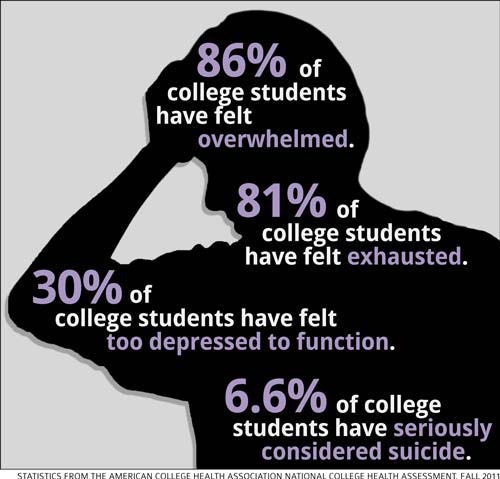
\includegraphics[width=0.3\textwidth]{img/mental-health.png}
  \caption{\label{fig:frog1}\href{https://www.change.org/p/university-students-mental-health-days-for-college-students}{Mental Health (2011)}}
\end{wrapfigure}

\subsection{Introduction}
The goal of this project is to design an \textbf{Android app} that reduces the stress an average university
student experiences and assist them in managing their schedule.
As reported by a \href{https://www.thenationalstudent.com/Student/2017-08-31/82_of_students_suffer_from_stress_and_anxiety.html}{Uni Health study in the UK}, 82\% of students in higher 
education report symptoms of stress or anxiety.\\
According to an \href{https://www.theguardian.com/education/2019/may/31/why-are-students-at-university-so-stressed}{article by the guardian}, a large number of students 
experience poor work-life balance, which is ``a huge contributing factor to mental health issues and stress''.
This means that many students are unable to stay focused, be sufficiently productive 
or avoid procrastination. \\
\\
\\
This imbalance is known to lead to mental health issues such as:
\begin{description}
    \item[Sleep Disorder:] As students either fail to work efficiently to complete coursework 
    in time, or are unable to find a healthy work-life balance due to social or professional 
    pressure, sleep is often neglected.
    \item[Anxiety:] As students struggle to micro-manage the large number of tasks they are 
    expected to handle on a daily basis, they lose their feeling of self-control. This can 
    lead to a variety of mental health issues including anxiety but can lead as far 
    as \textbf{panic attacks, depression} or \textbf{suicidal thoughts}.
\end{description}
\ \\
The Mental Health Tracking app tries to battle these issues, which, if not addressed properly early on, 
can permanently damage individuals in their ability to live a healthy life and achieve future endeavours.\\

Our app aims to allow University of Birmingham’s students to spend more time on the important tasks in 
their university life. It allows them to easily organise their day by automating a large part of their 
schedule minimal user input.  
Using tracked data of the user, the application additionally proposes assistance and advice if it 
detects potential for improvements to their lifestyle and rewards the user for reaching their goals. 

This gives valuable time back to the user and gives them a feeling of being in control. The scope 
of this app is addressed below along with the assumption made about other APIs the app wishes 
to interact with.
\newpage
\subsection{Scope}
All functionalities of the mental health app are accessible when the user logs into the app after they 
have created an account. As such, information about the user made available to the app includes:
\begin{itemize}
    \item Name
    \item Email
    \item Phone number
    \item Preferences (recorded by a questionnaire within the sign-up process)
\end{itemize}
If given access to the user's university or canvas account, it will be able to access, extract and use 
the information below:
\begin{itemize}
    \item University schedule (Tom Moses University Schedule API)
    \item Assignment deadlines and related events (Canvas API)
\end{itemize}

The user can also choose to give their preferences based on their classes found in the calendar, 
and the assignments found in canvas.
For assignments with deadlines, the user can tell the system how long they think they will need 
to complete this tasl.
Otherwise the system will allow a set default value for time allocated each week to the task. 

The user will be able to use the app without needing credentials for either of their university account 
or their canvas account. However, doing so will limit the immediate functionality of the provided 
Intelligent Behaviour Analysis AI (IBA) for scheduling.
\\
\\
The app will collect extra information on the preferences of the user within the questionnaire. IBA will make recommendations based on these which the user can choose to edit and/or remove. The questionnaire will ask them about:
\begin{itemize}
    \item When and how long does the user want to sleep
    \item Procrastination habits
    \item Time spent on grocery shopping
    \item Time spent on social activities
    \item Time to get ready in the morning
    \item Exercising goals
    \item Specific routines
\end{itemize}

The AI will take in all the above timing information and attempt to shuffle them within the calendar in an efficient manner, the result of which will be the base schedule every new user will be greeted with. As the user continues to interact with the app, they will be actively recommended modifications based on new inputs. The user can selectively choose which changes to include in their schedule.
\newpage
Every day when the user first logs in, the app will ask them simple questions, such as for how long have they slept. The AI will then recommend a longer sleep time if the user recorded low sleep the previous day. 


All collected inputs are stored locally and on the cloud servers to help sync across all user devices. As such, all transfer of information must be done securely and efficiently.
The AI will plan for a month at a time. This accounts for uncertainty within students’ actual schedules during the weeks and to compress user info synced to the cloud servers. 

As information is sent to a shared cloud with other accounts, potential issues to concurrency and scalability should be considered, as all users will upload their data to the servers. 
Therefore, the servers will handle all accounts’ synchronisation requests in a reliable and efficient manner.

\subsubsection*{Assumptions for the app}
\begin{itemize}
    \item The user of the app must create an account with a valid email to be able to receive periodic notification, and verify its account. 
    \item It is assumed that data transfer is scalable proportional to users once the system is set in place as new features may be introduced, increasing data transfer size. 
    \item It is assumed that the user will provide their own information, either manually setting their own calendar, or giving the app their preferences and letting the system set the calendar for them.
    \item It is assumed that IBA will always produce an efficient calendar catered to the user’s needs and preferences depending on the amount of information the user enters.
\end{itemize}

\newpage

\hypertarget{requirements-analysis}{%
\section{Requirements Analysis}\label{requirements-analysis}}

\hypertarget{functional-requirements}{%
\subsection{Functional Requirements}\label{functional-requirements}}

\hypertarget{cloud-based}{%
\paragraph{1. Cloud-based}\label{cloud-based}}

\begin{itemize}
 
\item
  The local app will ensure the user will be able to retrieve their
  accounts and the contents from the cloud database onto a new device.

  \begin{itemize}
  \item
    The app must upload user data to server to sync user account
    information across the number of devices the user is using.
  \item
    The app will upload all user data to server

    \begin{itemize}
     
    \item
      The app will upload questionnaire answers and preferences.
    \item
      The app will upload user-collected information.
    \item
      The app will upload API and login credential information.
    \end{itemize}
  \item
    The app will fetch user data from server
  \item
    The app will fetch data from connected APIs

    \begin{itemize}
     
    \item
      The app will download new changes from the user's \textbf{Bham}
      calendar if given account credentials. (see: 6. Account
      Management)
    \item
      The app will download new changes from the user's \textbf{Canvas}
      account if given account credentials. (see: 6. Account Management)
    \end{itemize}
  \item
    The app will resolve changes between devices to prevent conflicts
    with information
  \item
    In case of unreachable to cloud server, will attempt upload once
    re-established connection.
  \end{itemize}
\end{itemize}

\hypertarget{registration-and-login}{%
\paragraph{2. Registration and Login}\label{registration-and-login}}

\begin{itemize}
 
\item
  The user will not be able to access the main functionalities of the
  app until they have either logged in or signed up for an account to
  log in.

  \begin{itemize}
   
  \item
    The app will check if there is an account registered and log in,
    otherwise, the user will be directed to a log-in screen and has the
    option to create an account.

    \begin{itemize}
     
    \item
      The user will log in with their credentials - email and password.
    \item
      Upon loggin in, the user will choose to save credentials for
      automatic login next time they start the app.
    \item
      For security reasons, user credentials are stored in the cloud
      (see: 1. Cloud-based) as well as locally.
    \item
      New password resets will be uploaded to the cloud, which is
      compared against locally saved password.
    \item
      The unchanged local password will fail from now on when being
      compared to new credentials on the cloud server.
    \end{itemize}
  \item
    When signing up for an account, the app will direct them to a new
    screen.

    \begin{itemize}
     
    \item
      The user must provide the app with their credentials (email and
      password), and then a confirmation email will be sent to their
      email address in order to confirm the user-email.
    \item
      The user must confirm the email to verify registration.
    \item
      The user can provide the app with their Bham credentials and if
      done so:

      \begin{itemize}
       
      \item
        The app will extract the information regarding schedule from
        their Bham account, and insert it into the calendar (see: 3.
        Calendar)
      \end{itemize}
    \item
      The user can provide the app with their Canvas credentials and if
      done so:

      \begin{itemize}
       
      \item
        The app will extract information regarding deadlines and will
        add it to the calendar and todos (see: 3. Calendar, 4.Todo)
      \end{itemize}
    \item
      The user can provide their personal information through a
      questionnaire as part of the sign-up process. The user can choose
      to skip any of the given questions.

      \begin{itemize}
       
      \item
        The questions from the questionnaire will be used to tailor the
        Behaviour Analysis AI output to the user needs. (see: 7. AI)
      \end{itemize}
    \item
      The user will be able to add or remove personal information in
      their account management after signup (see: 6. Account Management)
    \end{itemize}
  \item
    If the user has an account but has forgotten the password, they can
    opt to reset password by receiving a change password hyperlink to
    the email they used to register their account with.
  \end{itemize}
\end{itemize}

\hypertarget{calendar}{%
\paragraph{3. Calendar}\label{calendar}}

\begin{itemize}
 
\item
  The user will be able to modify the calendar upon signing into their
  account.

  \begin{itemize}
   
  \item
    The user can add an event given all required information on name,
    date and length, with length 0 being a deadline event.
  \item
    The user can provide additional information on the event

    \begin{itemize}
     
    \item
      location of event
    \item
      the pattern of the event of if it is a recurring event.
    \end{itemize}
  \item
    The user can delete an event, duplicate the event, or edit any
    sub-information belonging to the event.

    \begin{itemize}
     
    \item
      the user will be able to specify if they are modifying for all
      subsequent events of the same name, or just the instance of the
      chosen event.
    \end{itemize}
  \end{itemize}
\item
  The calendar will be modified by fetching calendar information from
  Bham and Canvas if given access by user.

  \begin{itemize}
   
  \item
    The app will have access to modification rights as if it was another
    user.
  \item
    The app will not consult user on adding events taken from the
    external sources, but the user is able to treat them as user-added
    events and modify them.
  \end{itemize}
\item
  The app will attempt to modify the calendar (the user can reject the
  changes) based on user-collected information from both the trackers
  (see: 5. Tracker) and personal information given from questionnaire
  (see: 6. Account Management) using the integrated AI (see: 7. AI).

  \begin{itemize}
   
  \item
    The calendar will receive recommended output from AI based on given
    information to schedule the calendar with daily tasks (such as
    exercise, study etc.).
  \item
    The user can choose to accept none to all of the recommendation the
    AI makes.
  \item
    The AI will offer only 2 weeks worth of event recommendations
    because it needs to account for changes in the already existing
    schedule which can lead to uncertainty.
  \end{itemize}
\end{itemize}

\hypertarget{todo}{%
\paragraph{4. ToDo}\label{todo}}

\begin{itemize}
 
\item
  The todo acts as a daily representation of the calendar, and thus
  syncs information between itself and the Calendar.
\item
  It will display it in a phone-friendly format to allow user to better
  see task requirements for the day, in a focused manner.

  \begin{itemize}
   
  \item
    It will add User events, Calendar events, and AI events and display
    them for the user based on current date.
  \end{itemize}
\item
  The user can create/edit/delete a todo in the same manner as they can
  an event in a calendar (see: 3.Calendar)

  \begin{itemize}
   
  \item
    The new todo changes will be synced to calendar as an event.
  \end{itemize}
\end{itemize}

\hypertarget{tracker}{%
\paragraph{5. Tracker}\label{tracker}}

\begin{itemize}
 
\item
  The tracker will collect information from health trackers either
  built-in on device from applications, or external fitness trackers,
  and user input within the app if given.

  \begin{itemize}
  \item
    The app will request permission to access existing tracked
    information on device and extract health information.
  \item
    The user can input tracking data themselves to the app.
  \item
    The app will display data for different time intervals about user
    health.
  \item
    The app will ask the user to give tracking data on their daily
    activities, such as sleep lengths.
  \item
    The user can choose to edit tracking data.
  \item
    The information collected through the tracker will be passed onto
    the AI (see: 7. AI) to create recommendations to improve the user's
    health.
  \item
    The tracker will send notifications to user about their health
    progress.
  \end{itemize}
\end{itemize}

\hypertarget{account-management}{%
\paragraph{6. Account Management}\label{account-management}}

\begin{itemize}
\item
  The user will be able to review their account information, to either
  add, edit, remove information.

  \begin{itemize}
  \item
    The user can edit the questionnaire information that they provided
    when signing up.
  \item
    The user can edit their credentials, password and emails to change
    them.
  \item
    The user can see all the devices that are accessing the account.
  \item
    The user can log out of the app, which transfer to log-in screen.

    \begin{itemize}
    \item
      The user can log out of all devices.
    \end{itemize}
  \end{itemize}
\item
  The user will be able to review and edit preferences regarding other
  functionalities of the app

  \begin{itemize}
  \item
    The user can choose to turn on or off the AI (see: 7.Behaviour
    Analysis AI)
  \item
    The user can choose to delete AI stored information about user.
  \item
    The user can choose to sync cloud data manually.
  \item
    The user can choose to set sync period, or disable sync. it'll be
    set to a default value otherwise.
  \end{itemize}
\item
  The app will be able to make use of the information given by the user.
  The user must be able to set how much information the app can use.
\end{itemize}

\hypertarget{intelligent-behaviour-analysis-ai-iba}{%
\paragraph{7. Intelligent Behaviour Analysis AI
(IBA)}\label{intelligent-behaviour-analysis-ai-iba}}

\begin{itemize}
\item
  IBA will create scheduling models based on collected information from
  other functionalities of the app that the user can access

  \begin{itemize}
  \item
    IBA collects information based on changes from the Calendar (see: 3.
    Calendar), User-given personal information (see: 6. Account
    Management), and from Tracker (see: 5. Tracker)
  \item
    IBA will attempt to sort the information coming in to produce an
    optimised schedule for a period of 2 weeks.
  \item
    IBA will recommend modifications to its own schedule model for the
    week based on actual user activity throughout the day collected from
    trackers (see: 5.Tracker).

    \begin{itemize}
    \item
      i.e.~recommends more sleep hours for the following day if User
      reports light sleep for the previous day.
    \end{itemize}
  \item
    IBA will change its recommendation models based on how much of the
    models it recommends are rejected or accepted in attempt to study
    user preferences.
  \end{itemize}
\item
  IBA can be switched on or off by the user in Account Management (see:
  6. Account Management)
\item
  IBA's saved preferences can be deleted by the user in Profile
  Management (see: 6. Account Management)
\end{itemize}
\newpage
\hypertarget{non-functional-requirements}{%
\subsection{Non Functional Requirements}\label{non-functional-requirements}}

\hypertarget{sync-perf}{%
\paragraph{1. Synchronisation performance:}\label{to-add}}

\begin{itemize}
\item
  The app shall upload user data to the server within 3 seconds
\item
  The app shall fetch user data from server within 3 seconds (based on
  \textgreater1MB/s download speed of user)
\end{itemize}

\hypertarget{security}{%
\paragraph{2. Security}\label{security}}

\begin{itemize}
\item
  The app will implement hybrid cryptography for secure data transfer
  between cloud server and local app process used by user.

  \begin{itemize}
  \item
    The app must ensure data communications with external sources are
    either local or also secure. Unless necessary, all communications
    are primarily between local app and cloud server.

    \begin{itemize}
    \item
      Tracker applications and devices will be accessed without using
      any interaction between local app and cloud server.
    \item
      Tracker devices that rely on Bluetooth technology must also
      encrypt all transfer of communication between the device and the
      app.
    \item
      Fetching calendar/deadlines information from Bham API and Canvas
      API rely on the security of the respective systems.
    \item
      Credentials must be encrypted before transferring to API to avoid
      access-points into app or respective accounts of Bham and Canvas.
    \end{itemize}
  \end{itemize}
\end{itemize}

\hypertarget{reliability}{%
\paragraph{3. Reliability}\label{reliability}}

\begin{itemize}
\item
  The app should be designed to account for possible errors and failures
  in the components and attempt to address it without hurting user
  experience or minimising it.

  \begin{itemize}
  \item
    The AI should be designed and stress tested in mind to handle any
    and all changes in the app components.
  \item
    The app should be designed to sync information from cloud coming
    from older versions of the app and updating the local app
    accordingly.
  \item
    Conversely, components within the local app must be designed so
    that, once newer versions of the app are introduced with changes to
    its components, it must be able to interpret information from older
    versions of app without error. The app will only modify information
    based on changes to component between versions.
  \end{itemize}
\item
  The cloud server should be designed with redundancy in mind, syncing
  with back-up server(s) after every set uploads from all users to
  account for possible failure from either servers.
\end{itemize}

\hypertarget{scalability}{%
\paragraph{4. Scalability}\label{scalability}}

\begin{itemize}
\item
  The app should be constructed that an increase of users does not
  adversely affect the user experience of the individual user.

  \begin{itemize}
  \item
    Be designed that additional servers can be added or removed
    seamlessly and proportionally handle requests from users as user
    base increases or decreases.
  \item
    Load balancers control server traffic to prevent server overload.
    Cloud server maintains control over sync request from local app, and
    can issue earlier sync requests to reduce expected spikes in data
    due to set upload time, or divert sync request to additional
    identical servers.
  \end{itemize}
\end{itemize}

\hypertarget{efficiency}{%
\paragraph{5. Efficiency}\label{efficiency}}

\begin{itemize}
\item
  Actions the users may take must take a minimal amount of processing
  time of 1 second within the app.

  \begin{itemize}
  \item
    Communications to external API i.e.~Canvas or Bham must not add on
    significant waiting time than based on the users internet connection
    speed.
  \item
    All background tasks should be done in the background and thus can
    take more time, but must finish as soon as possible

    \begin{itemize}
    \item
      Server syncs should compare information between local app and
      cloud server to upload the smallest possible data.
    \item
      Behavioural Analysis AI should minimise time complexity given
      increase in information coming in to efficiently create
      recommendation models.

      \begin{itemize}
      \item
        The BAI should compare incoming information with current one
        that it is actively using, and only pass new information to
        update recommendation models, rather than recreating them each
        time.
      \end{itemize}
    \end{itemize}
  \end{itemize}
\end{itemize}

\hypertarget{maintainability}{%
\paragraph{6. Maintainability}\label{maintainability}}

\begin{itemize}
\item
  The app should be able to operate with minimal human oversight

  \begin{itemize}
  \item
    The BAI should be able to run autonomously without direct user
    interaction and run effectively with any given amount of information
    collected.
  \item
    The cloud servers should be able to operate either indecently from
    other servers in case of required server maintenance and updates.
  \item
    The cloud server should be set up to accept sync requests from older
    versions of the app as it only handles incoming packages of user
    information.
  \end{itemize}
\end{itemize}

\hypertarget{accessibility-and-usability}{%
\paragraph{7. Accessibility and
Usability}\label{accessibility-and-usability}}

\begin{itemize}
\item
  All of the app should be able to be used effectively with minimal
  instructions, and is intuitive to the user. The app should also be
  accessible by people with disabilities.

  \begin{itemize}
  \item
    The design of the UI must take into account of colour blindness so
    that people with them are not confused.
  \item
    The questions asked by the questionnaire should be short,
    understandable, concise.
  \item
    General word descriptors of the app functionalities should be short,
    understandable, concise.
  \item
    Aim to display the app in mostly visuals instead of words.
  \end{itemize}
\end{itemize}

\newpage

\section{Use Case}
\subsection{Comprehensive Use Case Diagram}
\begin{center}
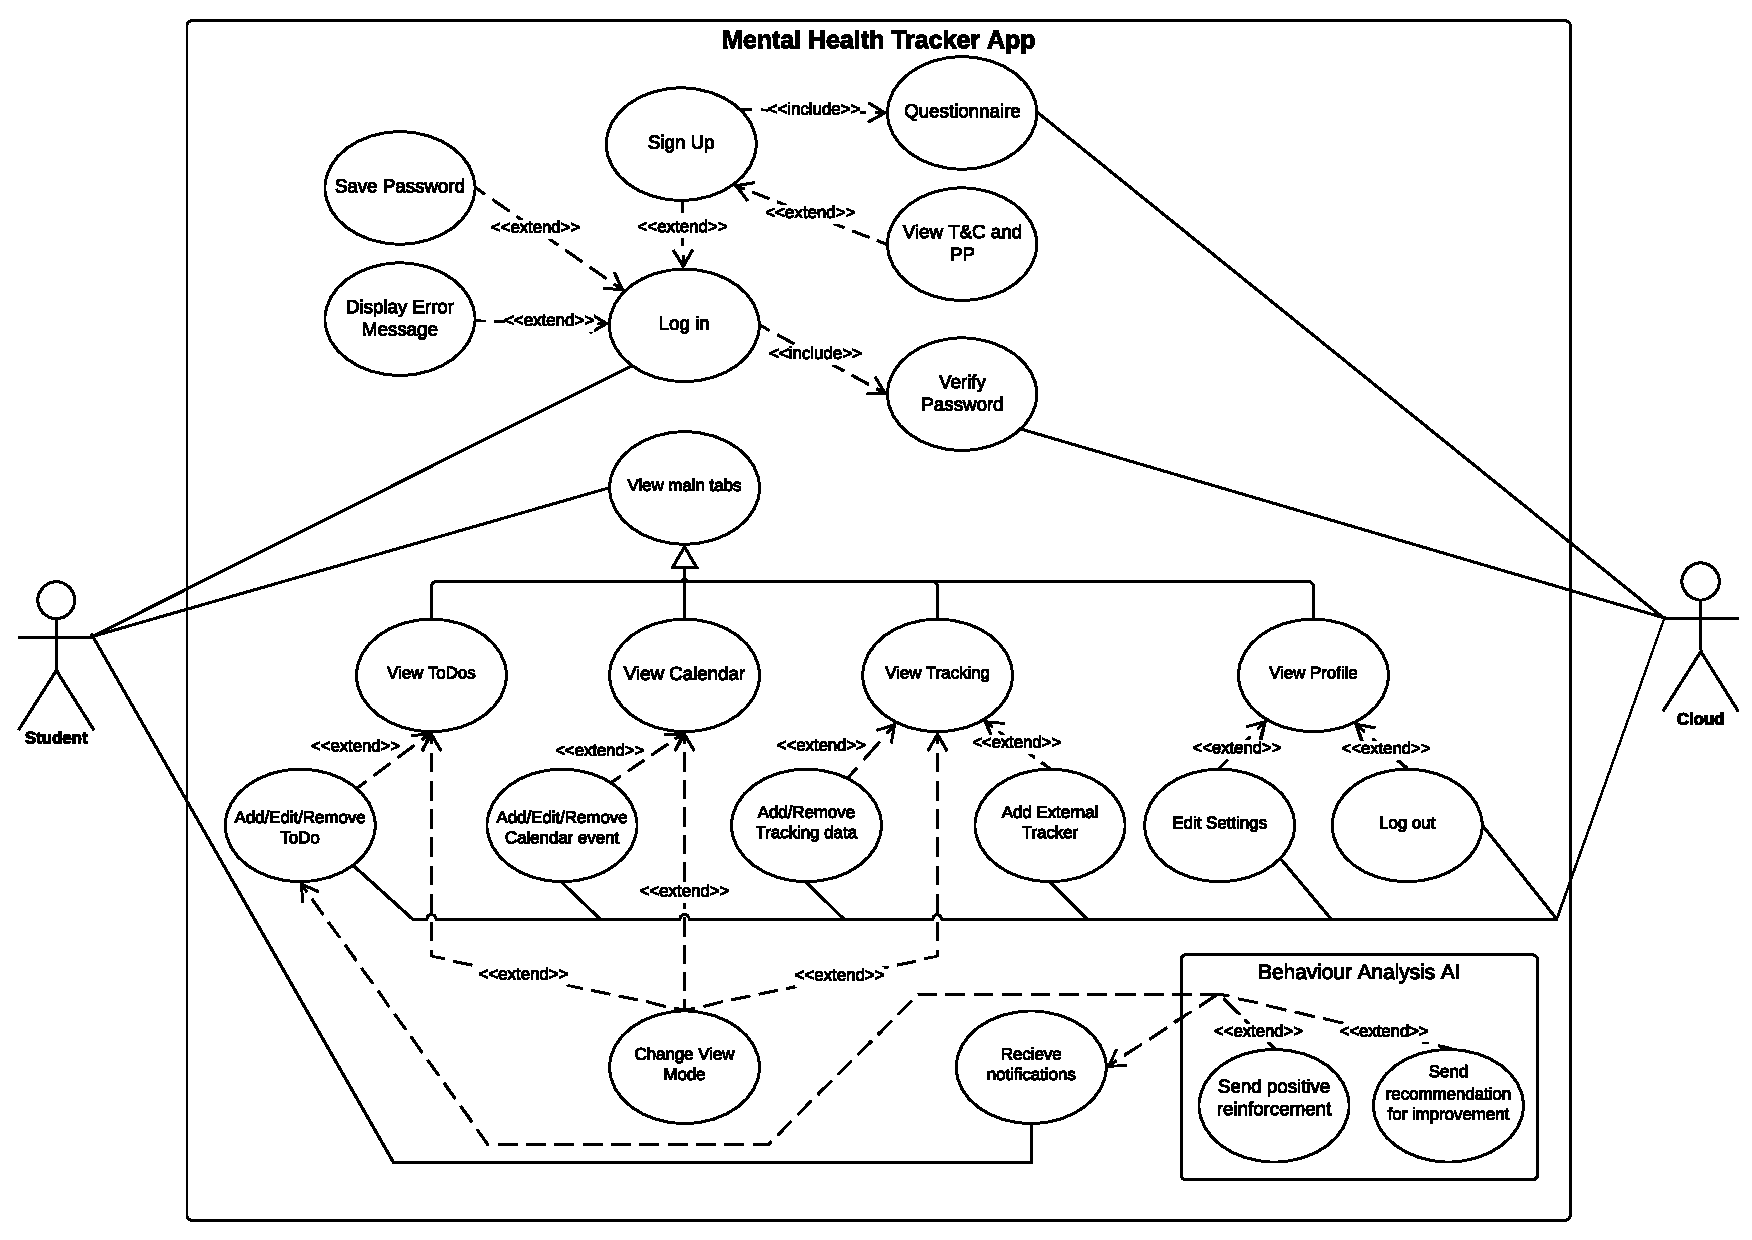
\includegraphics[angle=-90, scale=0.7]{img/Usecase_Diagram.pdf}
\end{center}
\subsection{Non-trivial Use Case: Add a tracker}
\subsubsection*{Precondition}
\begin{enumerate}
    \item User has created an account.
    \item User has logged into their account.
    \item User has selected tracker tab.
    \item (User selects add a tracker option from the tracker page.)
\end{enumerate}

\subsubsection*{Flow of Events}
\begin{enumerate}
    \item User selects Add a tracker option from the Tracking page.
    \item List of trackers that it is possible to import data from is shown to user.
    \begin{enumerate}
        \item If the user selects an item from the list, they are redirected to an authentication page.
        \item If the user selects cancel, then the user is asked to confirm their decision, after which they are returned to the tracker page or prompted to select a tracker from the list.
    \end{enumerate}
    \item Once on the authentication page the user will be asked to give permission to allow the app to access their data from the selected tracking service.
    \begin{enumerate}
        \item If the user accepts, they are shown a “gathering information” page
        \item If the user rejects the authentication they are returned to the list of trackers.
    \end{enumerate}
    \item Request is sent to the service the user selected
    \item \begin{enumerate}
        \item If the request is declined/fails user is shown a box which tells them the data import failed, and to try again later, then they are returned to the select tracker screen.
        \item If request is accepted, then a token is returned which is used to get data using the chosen services api.
    \end{enumerate}
    \item Request made to selected service.
    \begin{enumerate}
        \item If errors occur with the requests they are tried again x times, if continued errors the process will be cancelled and the user will be returned to the select a tracker screen and shown a message telling them an error occurred.
        \item If no errors occur, then the system continues.
    \end{enumerate}
    \item The data collected is put into apps databases etc to be viewable by the user in the app.
    \begin{enumerate}
        \item The data will be handled differently depending on the app it was collected from.
    \end{enumerate}
    \item User data stored on the cloud gets updated.
    \item Once the process is complete the user is returned to the select tracker page and told that the import was a success.
\end{enumerate}

\subsubsection*{Post Conditions}
\begin{enumerate}
    \item System updates the user’s information, using the new data imported from the added tracker, if a tracker was added.
    \item The system returns to an idle state and waits for the next input.
\end{enumerate}
 
 
\subsubsection*{Actors}
The user is the main actor in this use case as they will initiate the case by selecting the tracking tab in the app, and the tracking application that the data will be collected from. Another actor will be the cloud as the user data will be updated if the user makes any changes.

\subsubsection*{Scenarios}
\begin{enumerate}
    \item User A selects “Add a tracker” option from the tracker page and is prompted to select the tracker that they would like to import data from. They select Fitbit from the list of options. The user is redirected to the Fitbit OAuth 2.0 authorization page where the user selects “allow all” to give the app permission to collect all of their data from Fitbit. HTTP request is made to access the user’s data. User data is pulled from the server and imported to the in-app tracker. Data is added to local databases for use by other parts of the app etc. Data uploaded to cloud database. user is shown a message confirming their data has been imported and is returned to the selection screen.
    \item User B selects “add a tracker” option from the tracker page in is prompted to select the tracker that they would like to import data from. They select Fitbit from the list of options. The user is redirected to the Fitbit OAuth 2.0 authorization page where the user selects “deny all” User is sent back to the tracker page. System waits for user input.
\end{enumerate}
\newpage

\section{Activity Diagram}
\begin{center}
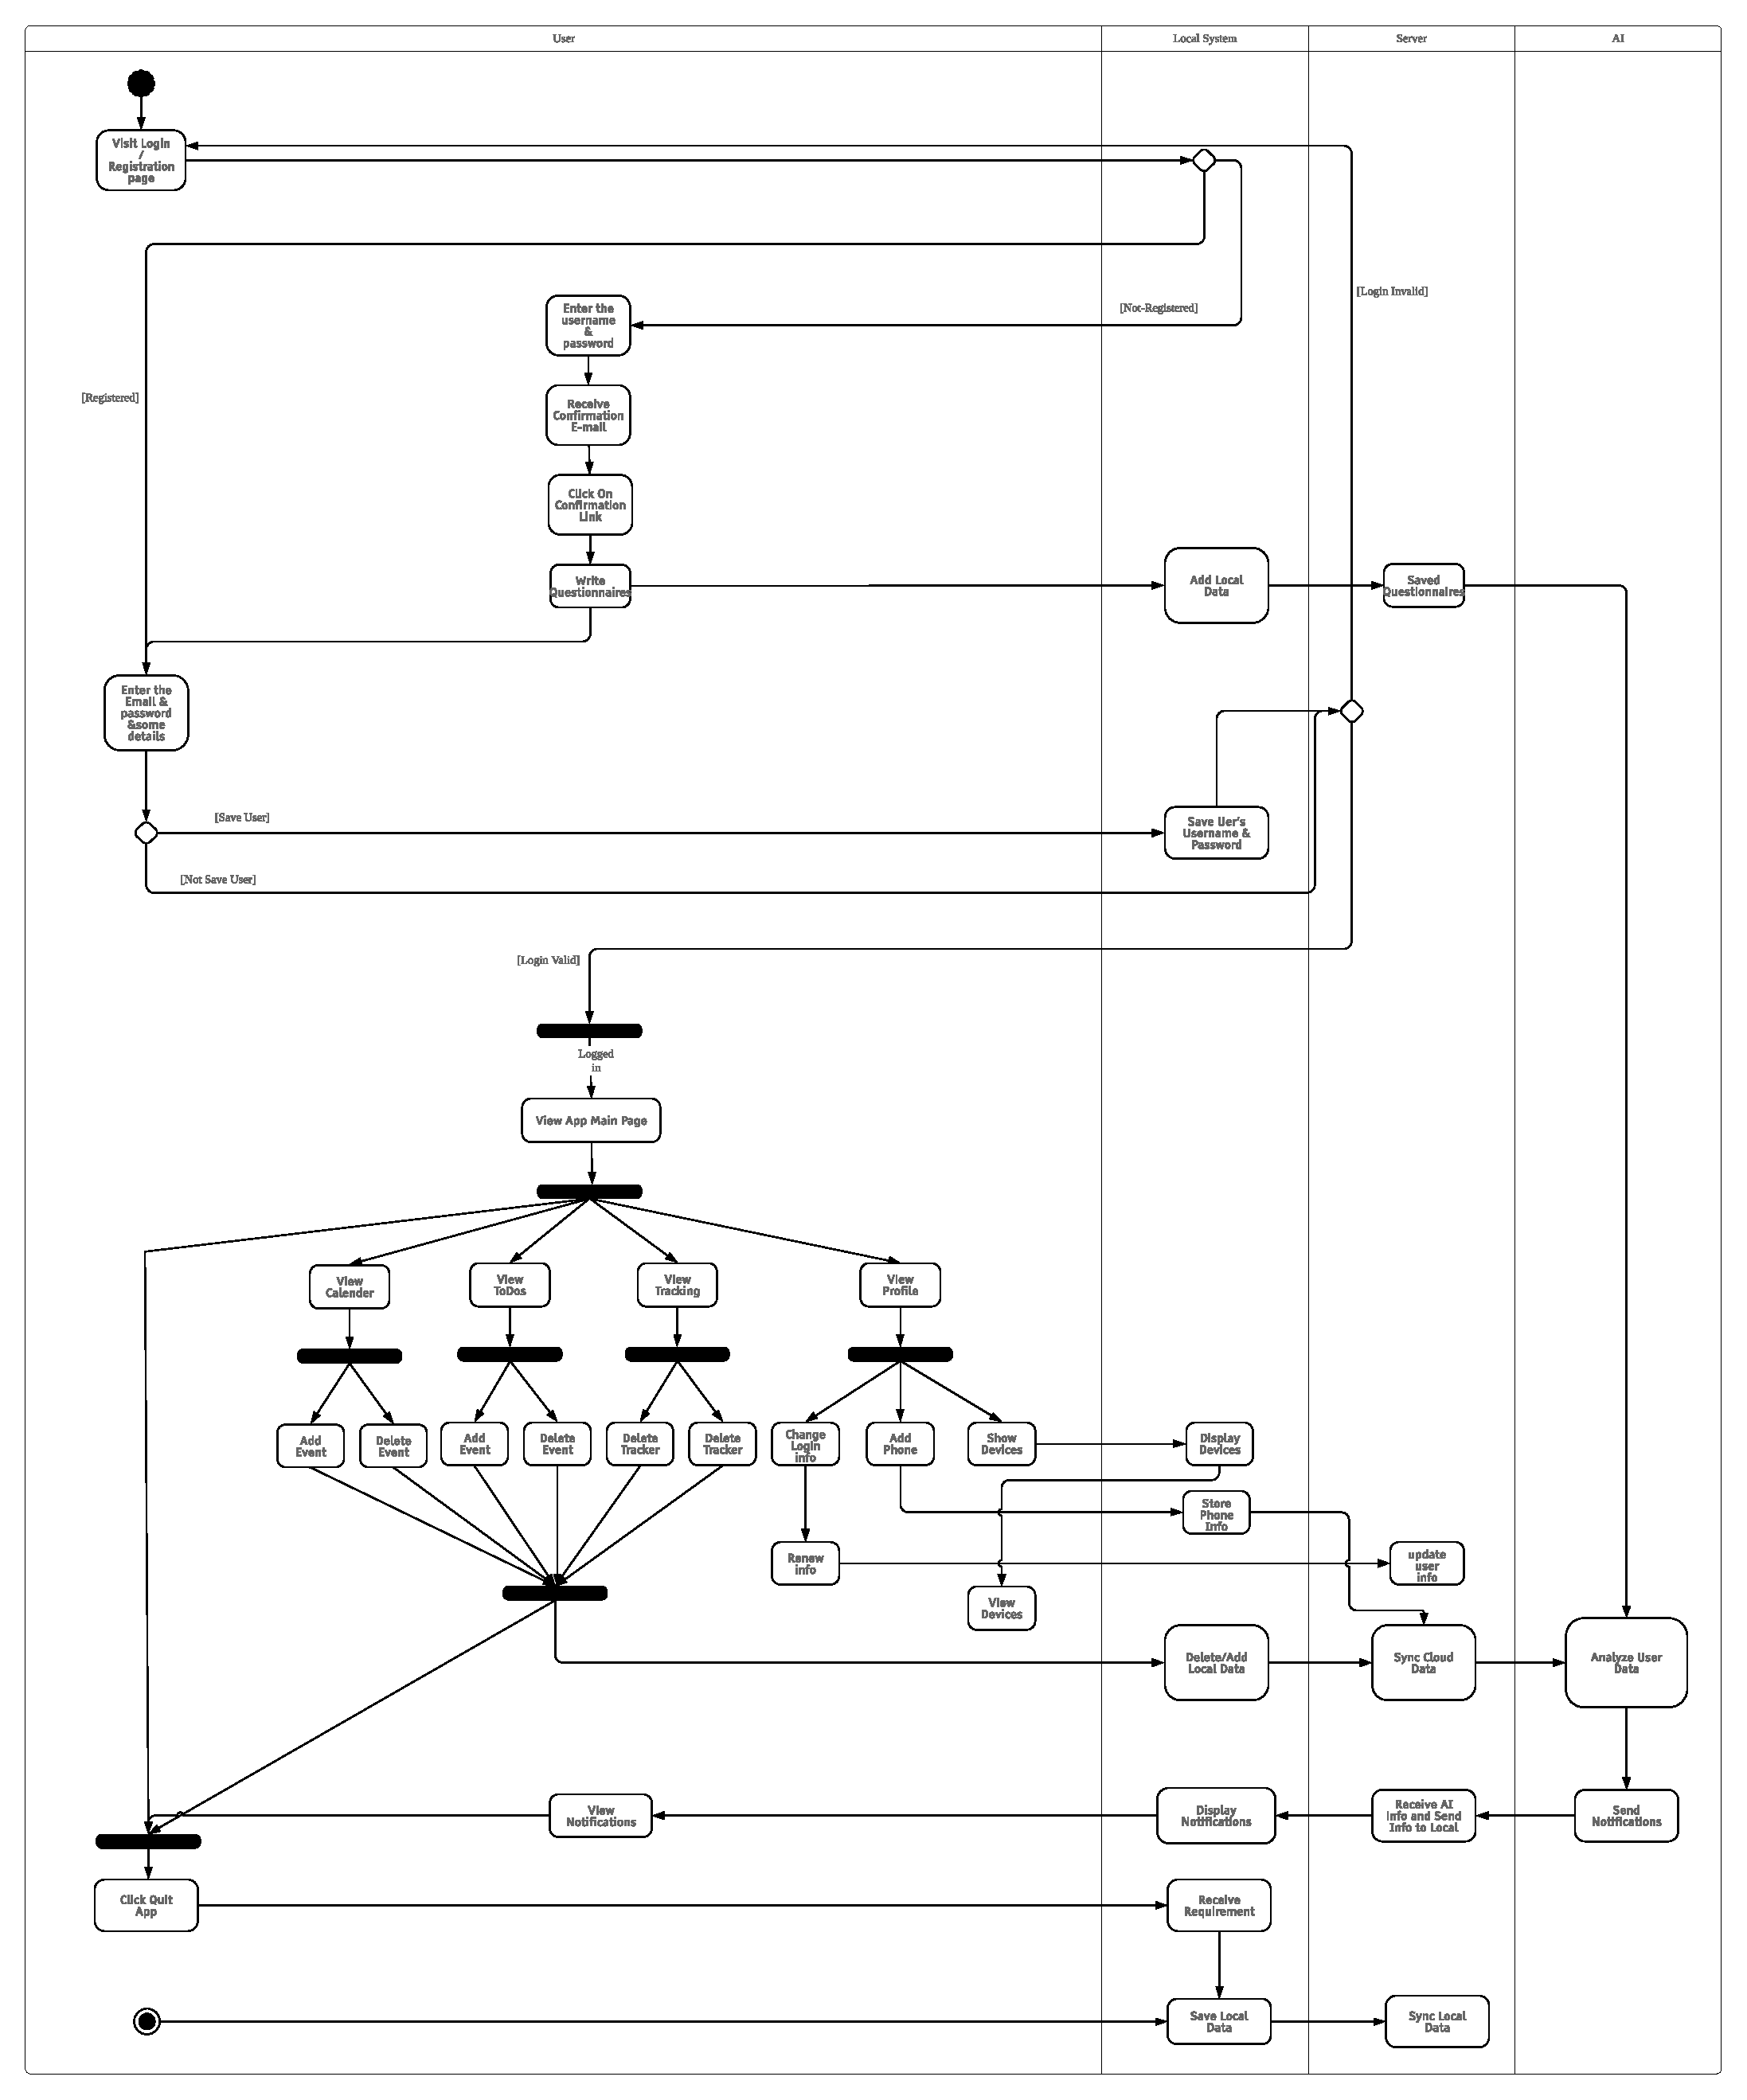
\includegraphics[width=\textwidth]{img/Activity_Diagram.pdf}
\end{center}
\newpage

\section{Class Analysis}
\subsection{Verb-noun Analysis}
\begin{description}
  \item[\textbf{Text}:] noun
  \item[\textbf{\underline{Text}}:] verb
\end{description}


\subsubsection*{1. Cloud-based}
\begin{itemize}
  \item The \textbf{local app} will ensure the \textbf{user} will be able to \textbf{\underline{retrieve their accounts}} and the contents from the \textbf{cloud database} onto a \textbf{new device}
  \begin{itemize}
    \item he app must \textbf{\underline{upload} user data} to server to \textbf{\underline{sync}} user account information across the number of devices the user is using
    \item The app will \textbf{\underline{upload user data}} to server within set time period
    \begin{itemize}
      \item The app will \textbf{\underline{upload new changes in the user's Bham calendar}} if given 
      \item The app will \textbf{\underline{upload new changes in the user's Canvas calendar}} if given 
      \item The app will \textbf{\underline{upload user-input personal information}}
      \item The app will \textbf{\underline{upload user-collected information}}
      \item The app will \textbf{\underline{upload up-to-date calendar configuration}}
    \end{itemize}
    \item The app will \textbf{\underline{fetch user data}} from server within set time period
    \item The app will \textbf{\underline{resolve changes}} between \textbf{devices} to \textbf{\underline{prevent conflicts}} \\\textbf{\underline{in information}}
    \item In the case of "unreachable to \textbf{cloud server}", it will \textbf{\underline{attempt to upload once}} \textbf{\underline{re-established connection}}.
  \end{itemize}
\end{itemize}


\subsubsection*{2. Registration and Login}
\begin{itemize}
  \item The user will not be able to \textbf{access} the main functionalities of the \textbf{app} until they have either logged in or signed up for an account to log in.
  \begin{itemize}
    \item The app will check if there is an account registered and log in, otherwise, the user will be directed to a \textbf{log-in screen} and has the option to \textbf{\underline{create an account}}.
    \begin{itemize}
      \item The \textbf{user} will log in with their \textbf{credentials}, email and password.
      \item Once logged in, the user can choose to \textbf{\underline{save credentials for automatic login}} next time they start the app.
      \item For security reasons, user credentials are \textbf{\underline{stored in the cloud}} as well as locally.
      \item \textbf{New password resets} will be \textbf{\underline{uploaded to the cloud}}, which is\\ \textbf{\underline{compared against locally saved password}}.
      \item Unchanged local password will fail once compared to new credentials recorded in cloud server.
    \end{itemize}
    \item When signing up for an account, the app will direct them to a new screen.
    \begin{itemize}
      \item The user must \textbf{\ul{provide the app with their credentials as email and password}}, of which a \textbf{confirmation email} will be sent to their account to affirm the existence of email account.
      \item The user can \textbf{\ul{provide the app with their Bham credentials}}, of which they will be asked to login to \textbf{\underline{confirm credentials}}.
      \begin{itemize}
        \item The app will \textbf{\ul{extract the information regarding schedule}} from their Bham account, and \textbf{\underline{insert it into the calendar}}.
      \end{itemize} 
      \item The user can \textbf{\ul{provide the app with their Canvas credentials}}, of which they will be asked to login to \textbf{\underline{confirm credentials}}.
      \begin{itemize}
        \item The app will \textbf{\ul{extract information}} regarding deadlines and add to the \textbf{calendar} and \textbf{todo}
      \end{itemize} 
      \item The user can \textbf{\ul{provide their personal information}} through the \textbf{questionnaire} as part of the \textbf{sign-up process}. The user can choose to answer any number of questions as to not turn the user away from the app by requesting this data to function.
      \begin{itemize}
        \item However, it is encouraged that the user provide the app which as much information as they are willing to.
        \item This allows the app to personalize the main component.
      \end{itemize} 
      \item The user will be able to \textbf{\ul{add or remove personal information}} in their \textbf{account management} after signup (see: 6. Account Management)    
    \end{itemize}
    \item If the user has an account but forgot the password, they can opt to \textbf{reset password} by sending it to the email they used to register their account with.
  \end{itemize}
\end{itemize}


\subsubsection*{3. Calendar}
\begin{itemize}
  \item The user will be able to \textbf{\ul{modify the calendar}} upon signing into their account.
  \begin{itemize}
    \item The user can \textbf{\ul{add an event}} given information on \textbf{name, date and length}, with length 0 being a deadline event.
    \item The user can provide additional information on the \textbf{event}
    \begin{itemize}
      \item \textbf{location of event}
      \item the pattern of the event of if it is a \textbf{recurring event}.
    \end{itemize}
    \item The user can \textbf{\ul{delete an event}}, \textbf{\ul{duplicate the event}}, or \textbf{\ul{edit any sub-information belonging to the event}}.
    \begin{itemize}
      \item the user will be able to specify if they are modifying for all subsequent events of the same name, or just the instance of the choosen event.
    \end{itemize}
  \end{itemize}
  \item The app will to \textbf{\ul{modify the calendar}} by \textbf{\ul{fetching calendar information from Bham}} and \textbf{Canvas calendar}, if given access by user.
  \begin{itemize}
    \item The app will have access to modification rights as if it was another user.
    \item The app will not consult user on adding events taken from the external sources, but the user is able to treat them as an user-added event.
  \end{itemize}
  \item The app will attempt to \textbf{\ul{modify the calendar}} based on user-collected information from both the tracker and personal information given from questionnaire
  \begin{itemize}
    \item The calendar will \textbf{\ul{receive recommended output from AI}} based on given information to schedule the calendar with \textbf{daily tasks}.
    \item The user can choose to accept none to all of the recommendation the AI makes, to commit to their weekly schedule.
    \item The AI will manage 2 weeks worth of recommendation of daily task, to account for changes in actual schedule which leads to uncertainty.
  \end{itemize}
\end{itemize}


\subsection*{4. ToDo}
\begin{itemize}
  \item The todo acts as a daily representation of the calendar, and thus \textbf{\ul{syncs information between itself and the Calendar}}.
  \item It will display it in a phone-friendly format to allow user to better see \textbf{\ul{task requirements for the day}}, in a focused manner.
  \begin{itemize}
    \item It will add \textbf{User events, Calendar events}, and \textbf{AI events} and \textbf{\ul{display}} them for user based on current date.
  \end{itemize}
  \item The user can \textbf{\ul{create/edit/delete a todo}} in the same manner as they can an event in a calendar (see: 3.Calendar)
  \begin{itemize}
    \item The new todo changes will be synced to calendar as an event.
  \end{itemize}
\end{itemize}


\subsubsection*{5. Tracker}

\paragraph{First time:}
\begin{itemize}
  \item \textbf{\ul{Request permission to access existing tracked information}} on device (e.g. Health apps)
\end{itemize} 

\paragraph{System can:}
\begin{itemize}
  \item \textbf{\ul{import tracking data}} from all permitted tracking applications
  \item \textbf{\ul{display progress}} for different time intervals (day, week, month, year)
  \item \textbf{\ul{perform tracking analysis}} to recommend user options of improvement (see: Tracker process)
  \item s\textbf{\ul{end reward notification}} when achieving goals
\end{itemize}

\paragraph{User can:}
\begin{itemize}
  \item \textbf{\ul{Add tracking data manually}} (e.g. [+] slept x hours)
  \item \textbf{\ul{Remove manually entered tracking data}}
\end{itemize}

\paragraph{Tracker process:}
\begin{itemize}
  \item \textbf{\ul{Create recommendation based on tracking AI}} (trained to recommend based on positive changes of the user?)
  \item \textbf{\ul{Send notification}} to user (e.g. slept sufficiently / caught up on sleep tonight)
\end{itemize}

\newpage
\subsubsection*{6. Account Management}
\begin{itemize}
  \item \textbf{\ul{Change account login details}} (email/password)
  \begin{enumerate}
    \item \textbf{\ul{Enter current and new}} email/password.
    \item UI to change credentials
    \begin{itemize}
      \item fields: old password, new password, confirm new password
      \item confirm and cancel box
    \end{itemize}
  \end{enumerate}
  \item \textbf{\ul{Add Phone}}
  \begin{enumerate}
    \item \textbf{\ul{Enter phone number}}
    \item \textbf{\ul{Verification code sent via sms}}
    \item \textbf{\ul{Enter verification code}}
  \end{enumerate} 
  \item \textbf{\ul{Show devices}}
  \begin{itemize}
    \item Show the user all the devices that are logged into the account
    \item allow user to \textbf{\ul{log out}} any of these devices so these devices must re-enter login details and get kicked out of current session
  \end{itemize} 
\end{itemize}

\subsubsection*{7. Intelligent Behaviour Analyser AI (IBA)}
\begin{itemize}
  \item IBA will \textbf{\ul{create scheduling models}} based on collected information from other functionalities of the app that the user can access
  \begin{itemize}
    \item \textbf{\ul{IBA collects information}} based on changes from the Calendar (see: 3. Caldendar), User-given personal information (see: 6. Account Management), and from Tracker (see: 5. Tracker)
    \item IBA will attempt to \textbf{\ul{sort the information}} coming in to \textbf{\ul{produce an optimized schedule}} for a period of 2 weeks.
    \item IBA will \textbf{\ul{recommend modification}} to it own schedule model for the week based on actual user activity throughout the day collected from tracker (see: 5.Tracker).
    \begin{itemize}
      \item i.e recommends more sleep hours next day if the user report short sleep the previous day.
    \end{itemize} 
    \item IBA will change its recommendation models based on how much of the models it recommend the user is rejected or accepted to study user preferences.
  \end{itemize}
  \item IBA must be able to be switched on or off by user, as well as its saved profile on user preferences be deletable.
\end{itemize}

\newpage
\begin{center}
    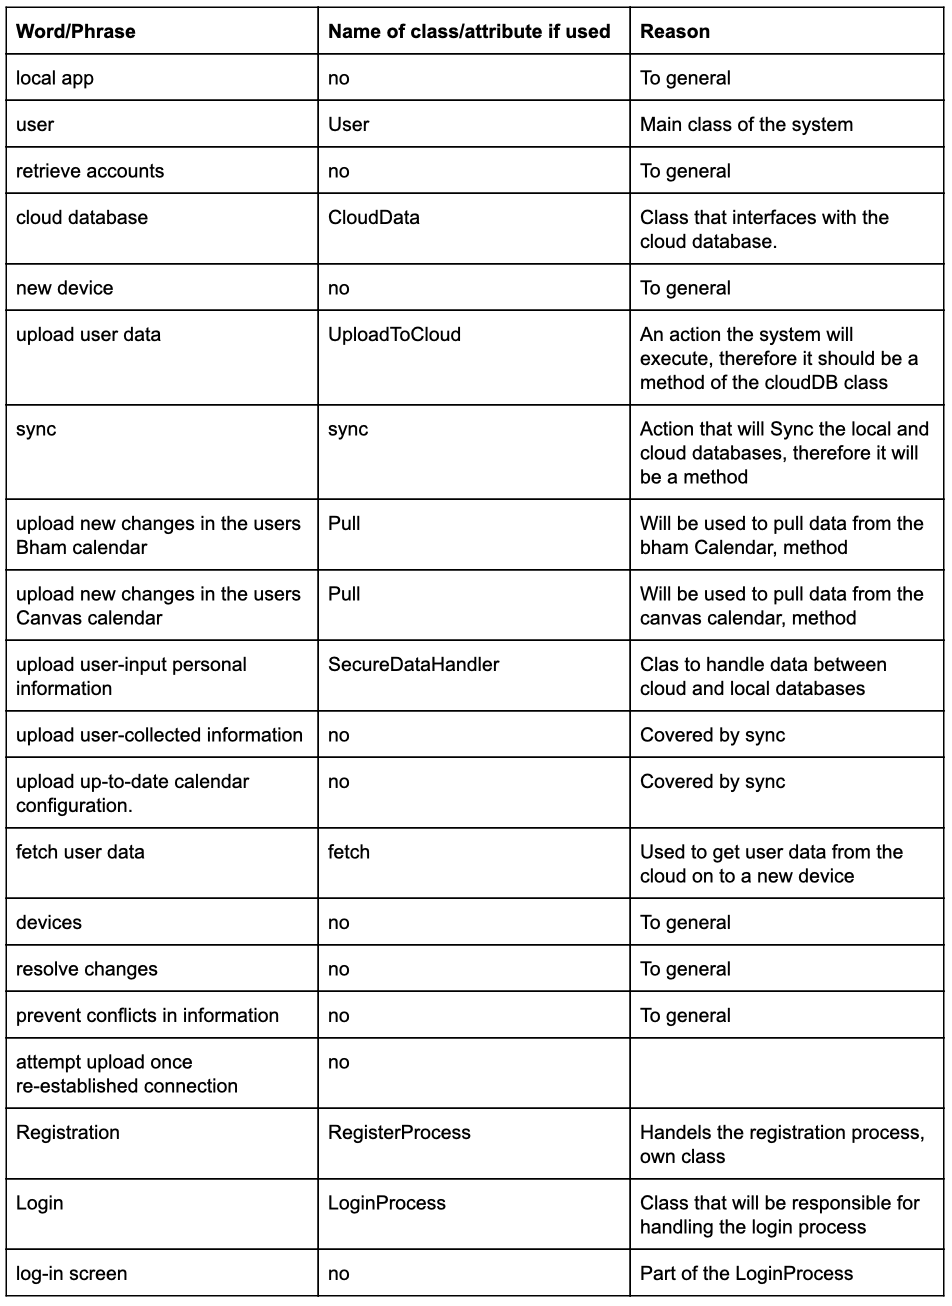
\includegraphics[scale=0.9]{img/noun-verb/table1.png}
    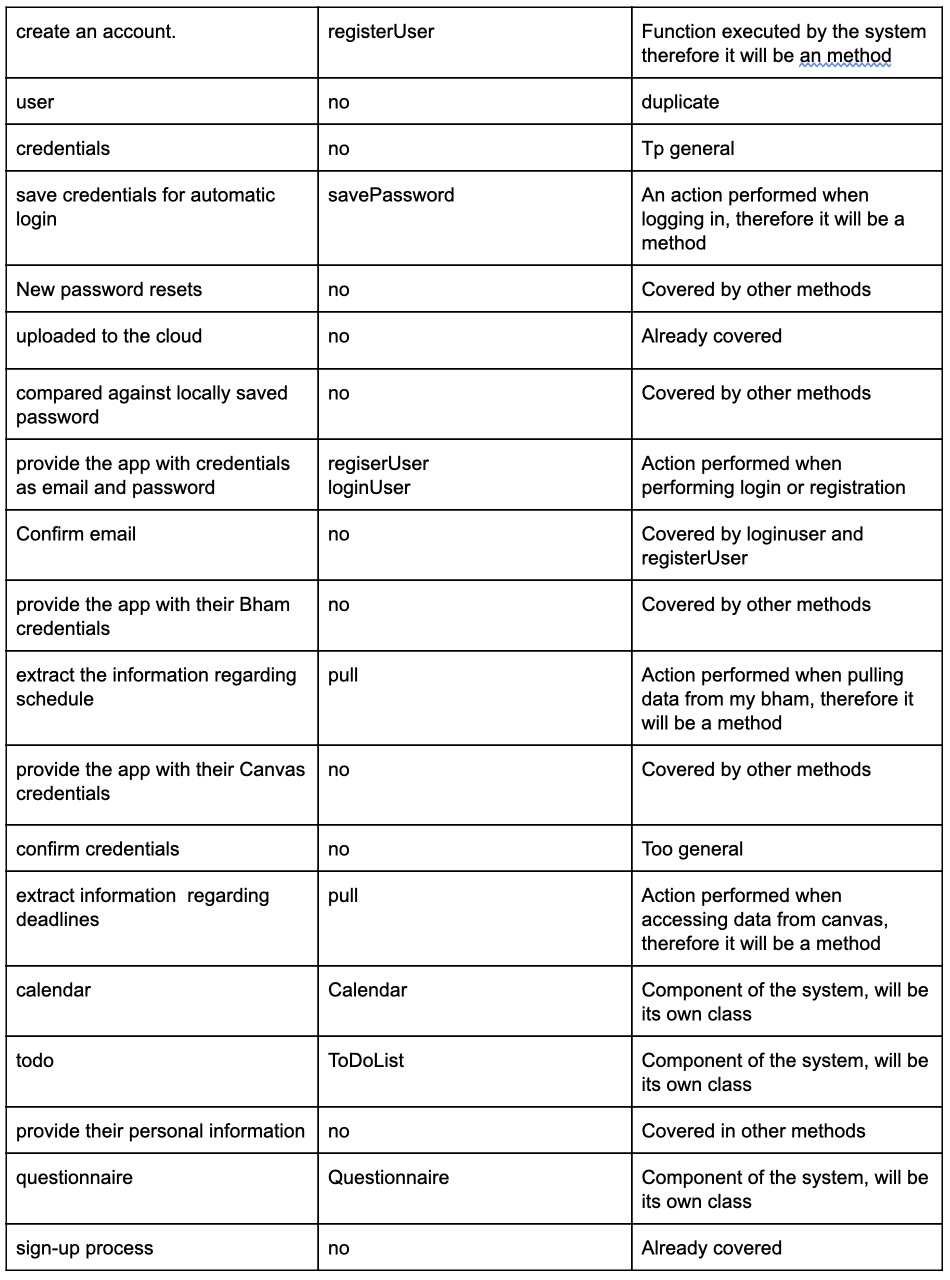
\includegraphics[scale=0.9]{img/noun-verb/table2.png}
    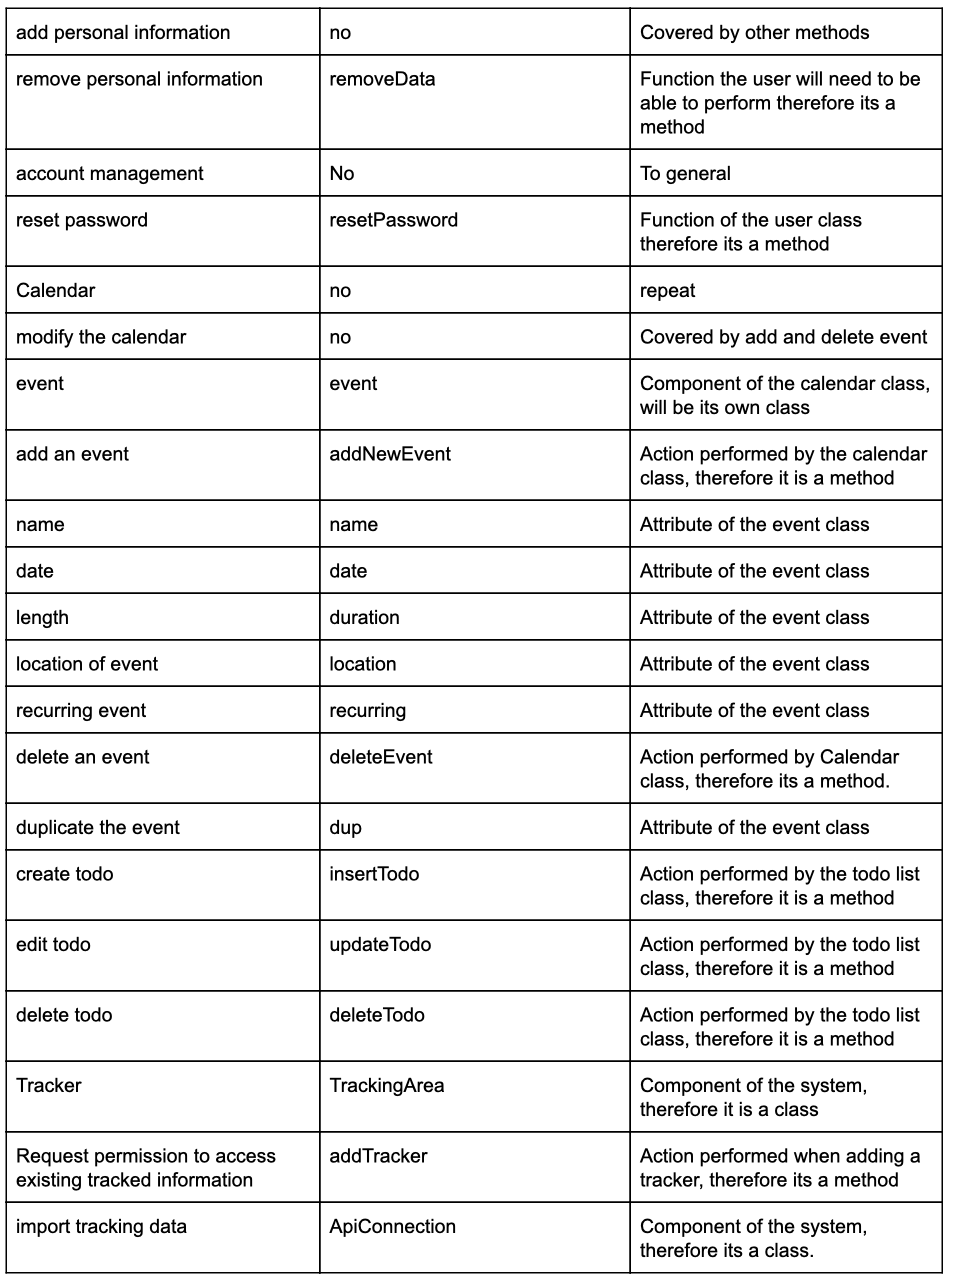
\includegraphics[scale=0.9]{img/noun-verb/table3.png}
    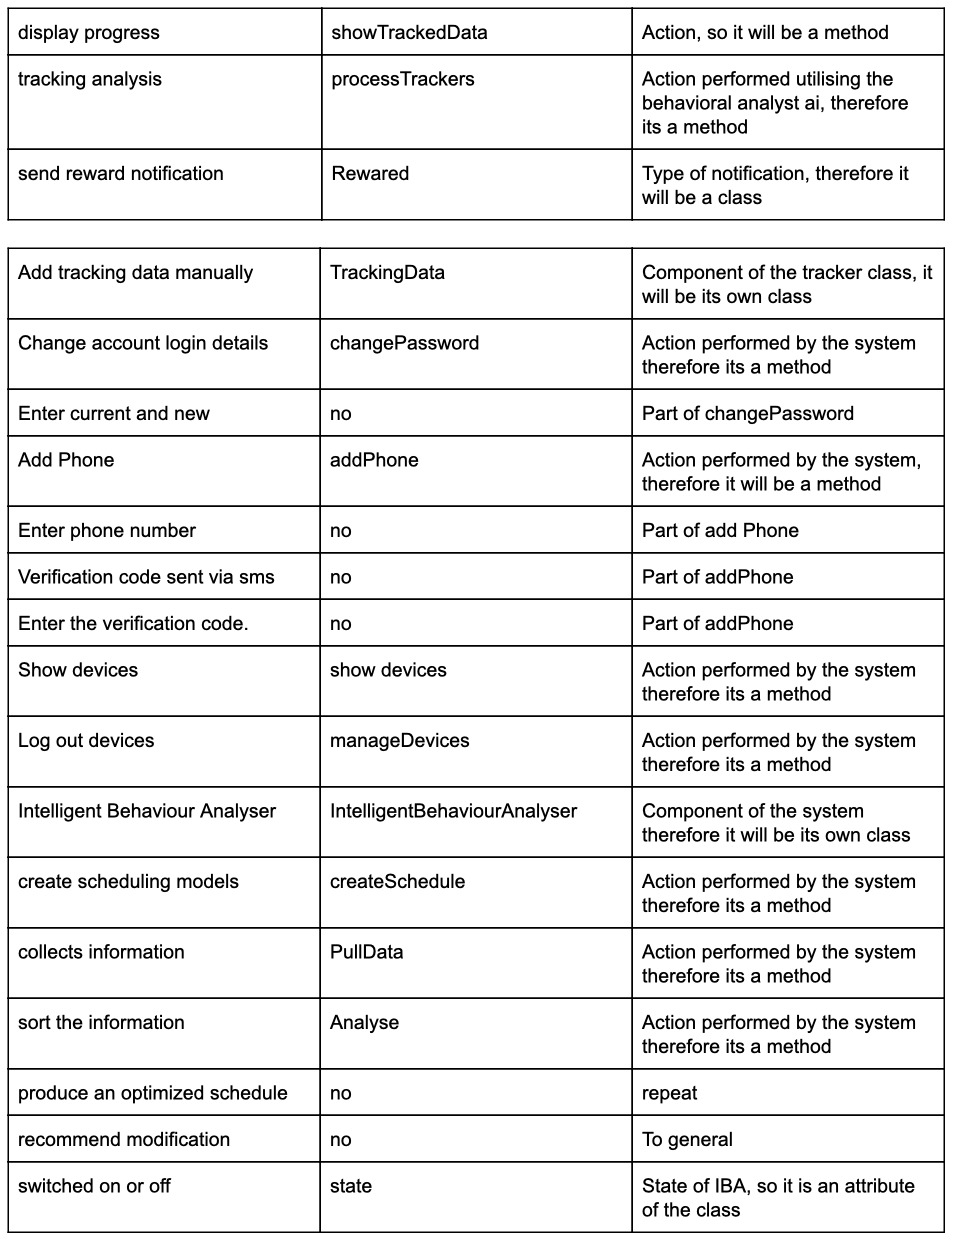
\includegraphics[scale=0.9]{img/noun-verb/table4.png}
\end{center}
\newpage
\subsubsection*{Responsibility Driven Analysis}
\vspace{1cm}
\begin{center}
  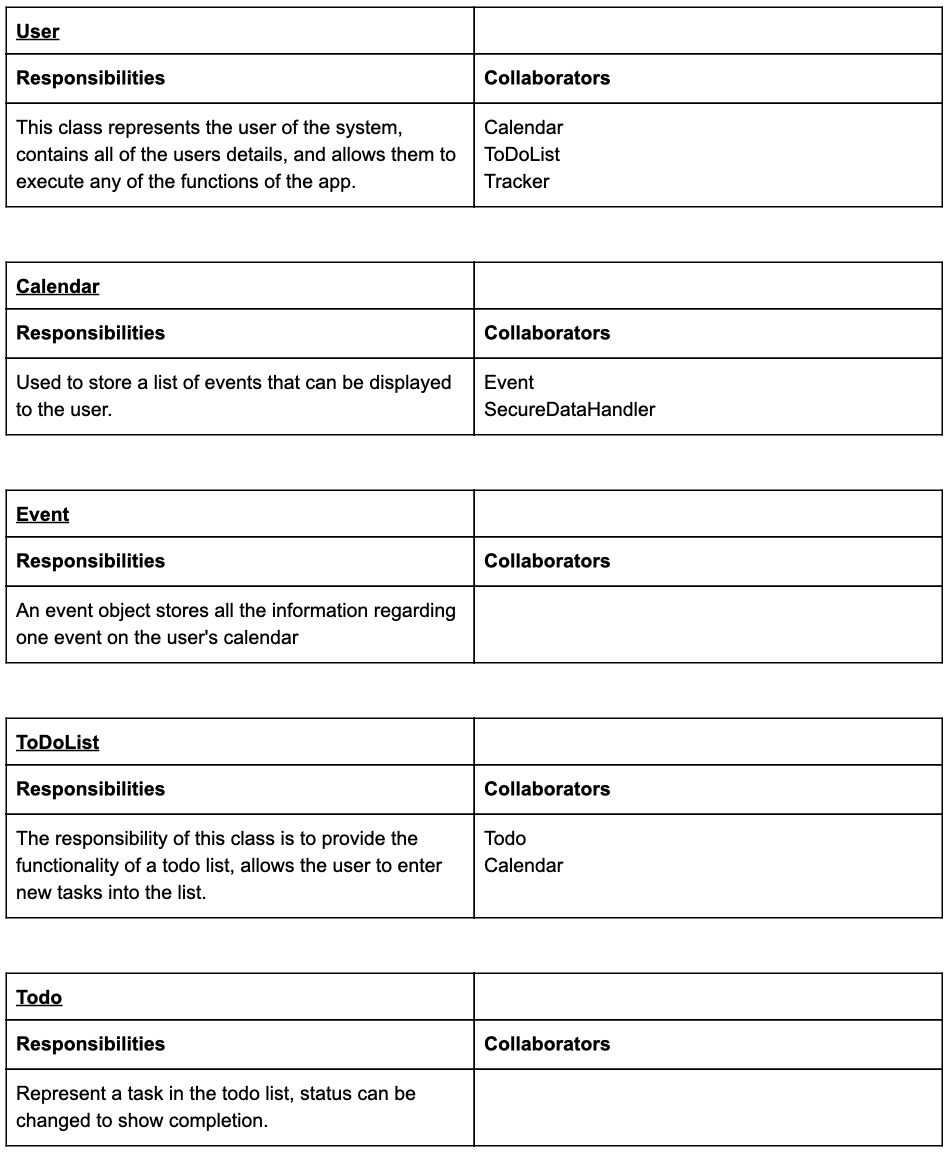
\includegraphics[width=\textwidth]{img/noun-verb/rda-table1.png}
  \newpage
  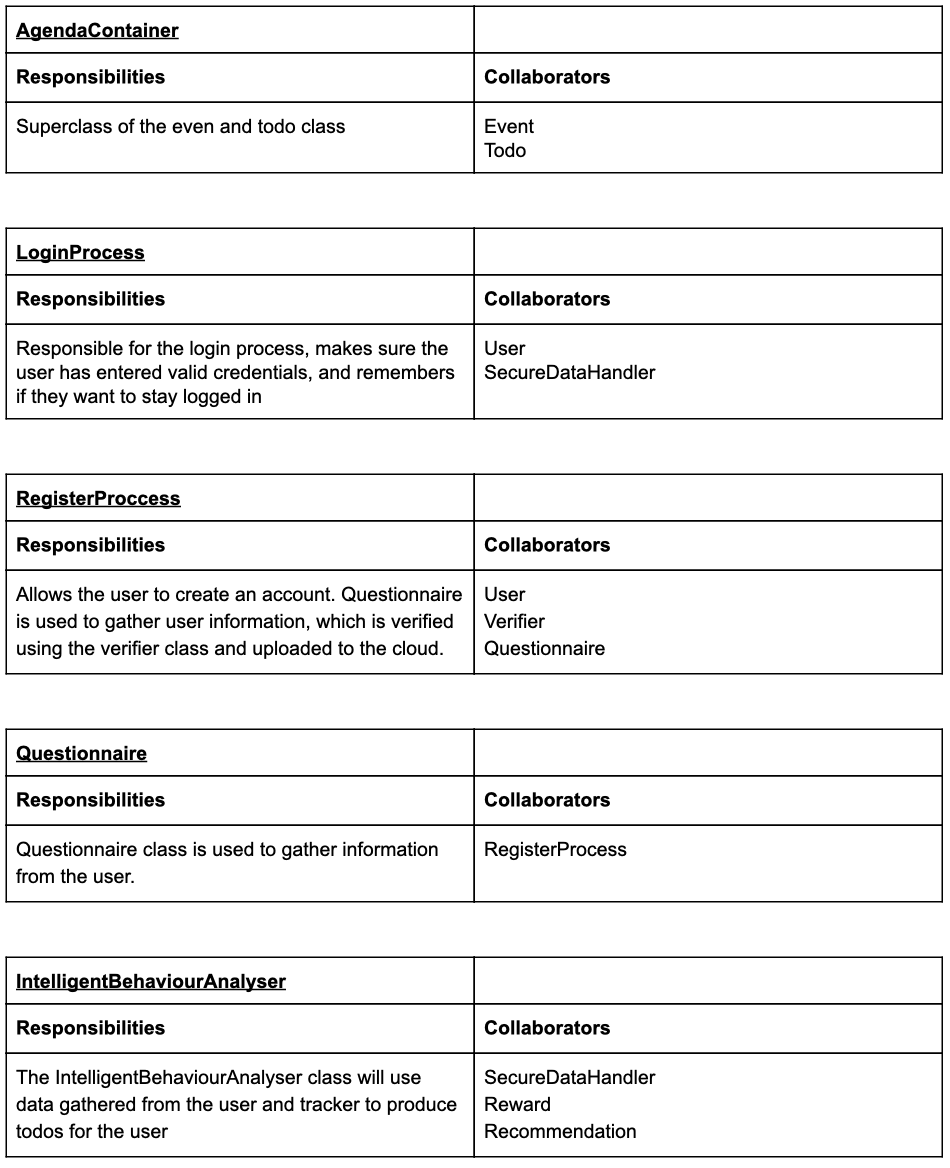
\includegraphics[width=\textwidth]{img/noun-verb/rda-table2.png}
  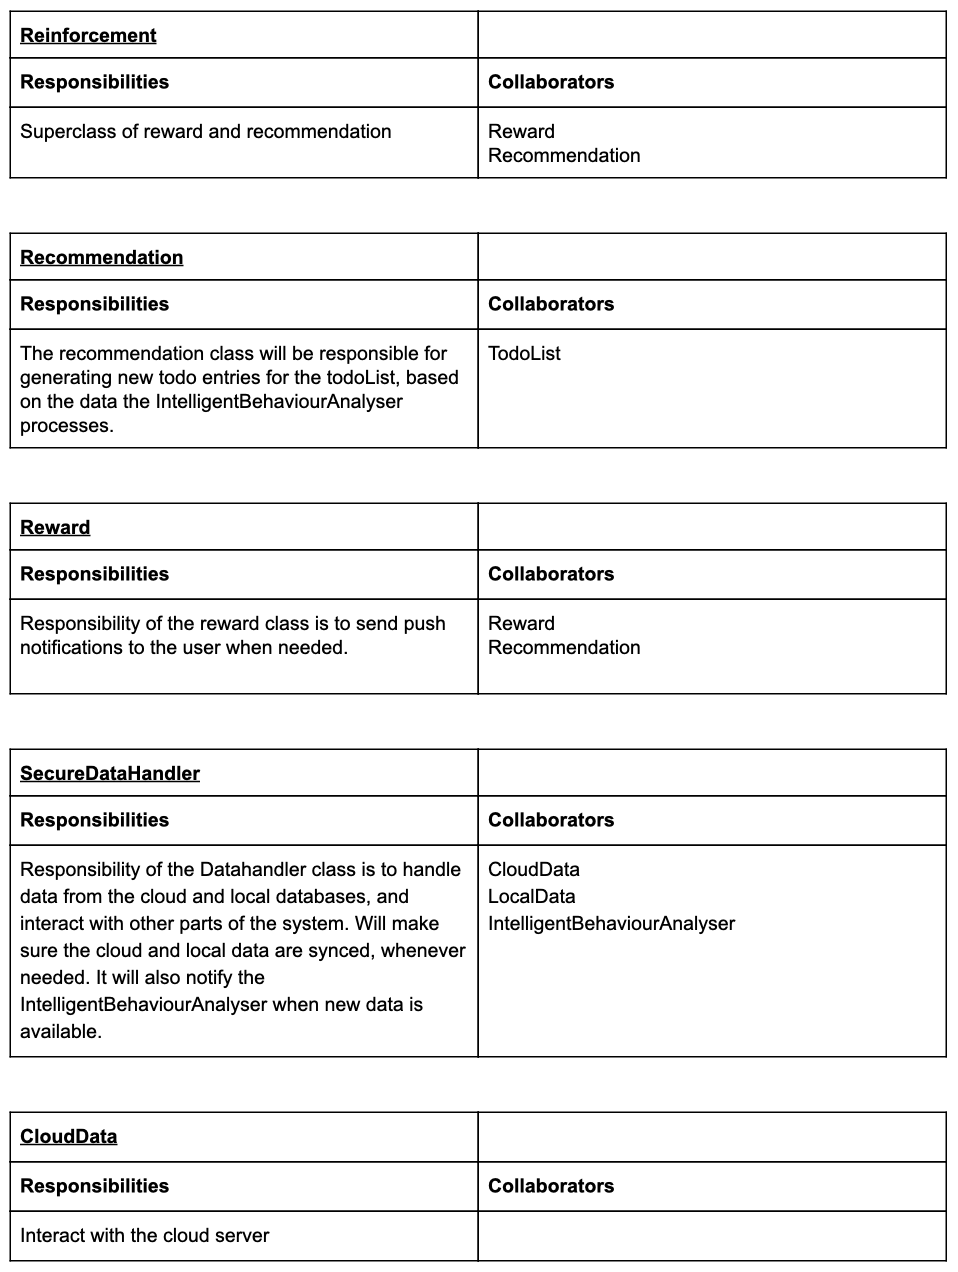
\includegraphics[width=\textwidth]{img/noun-verb/rda-table3.png}
  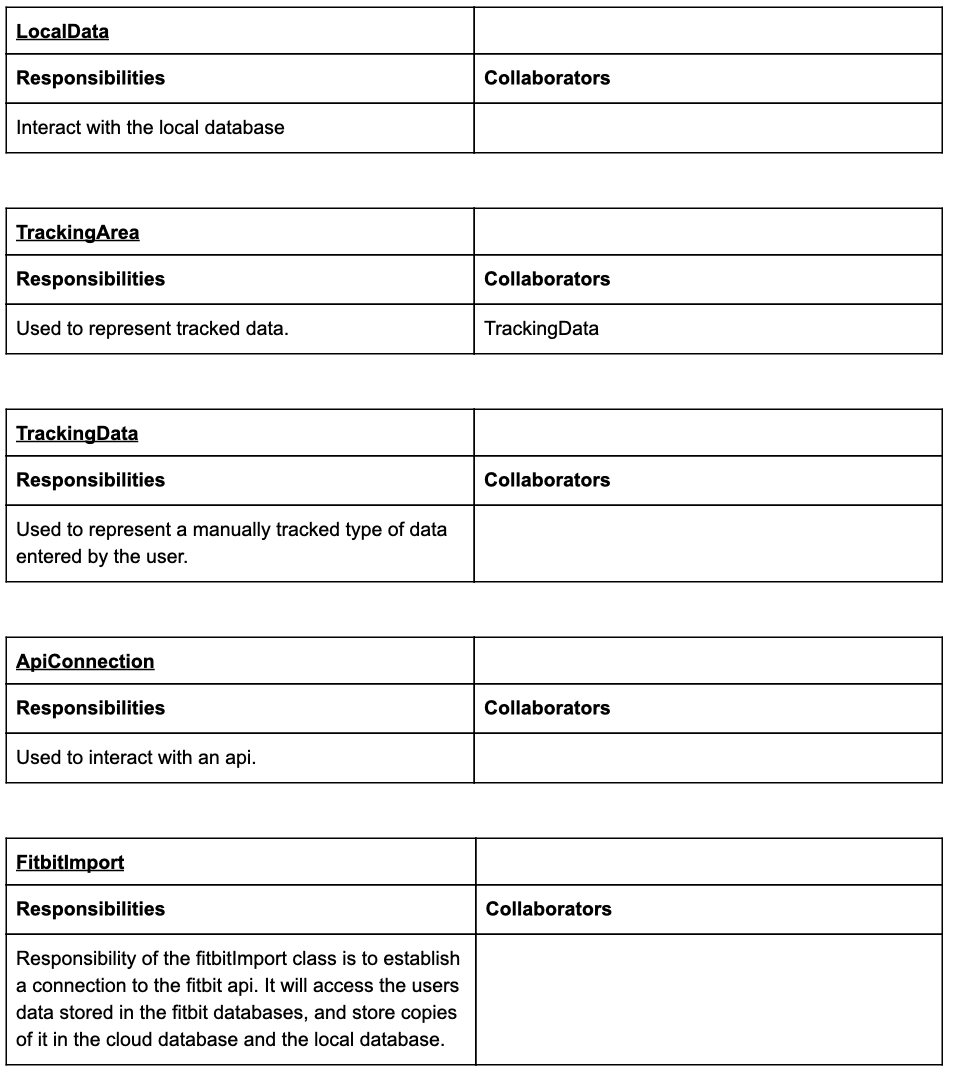
\includegraphics[width=\textwidth]{img/noun-verb/rda-table4.png}
  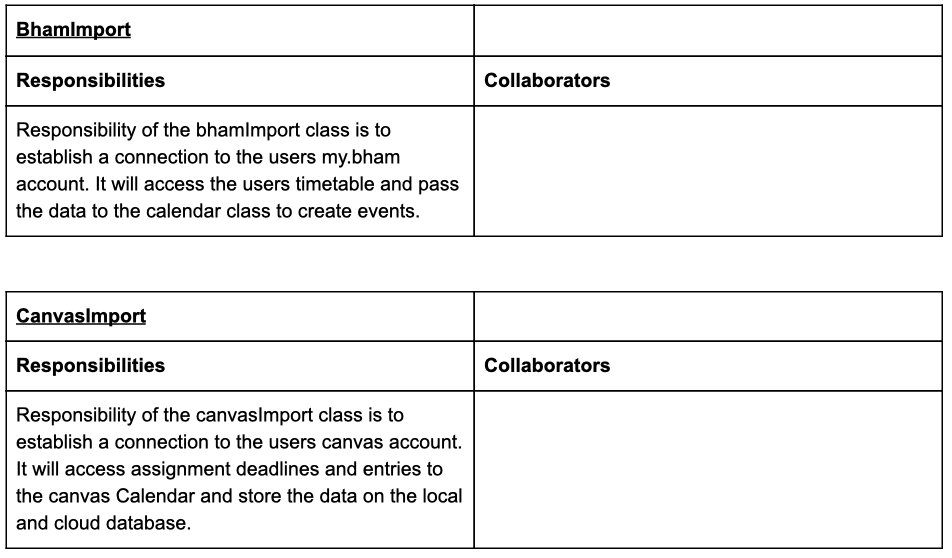
\includegraphics[width=\textwidth]{img/noun-verb/rda-table5.png}
\end{center}
\newpage

\subsection{First-Cut Class Diagram}
\begin{center}
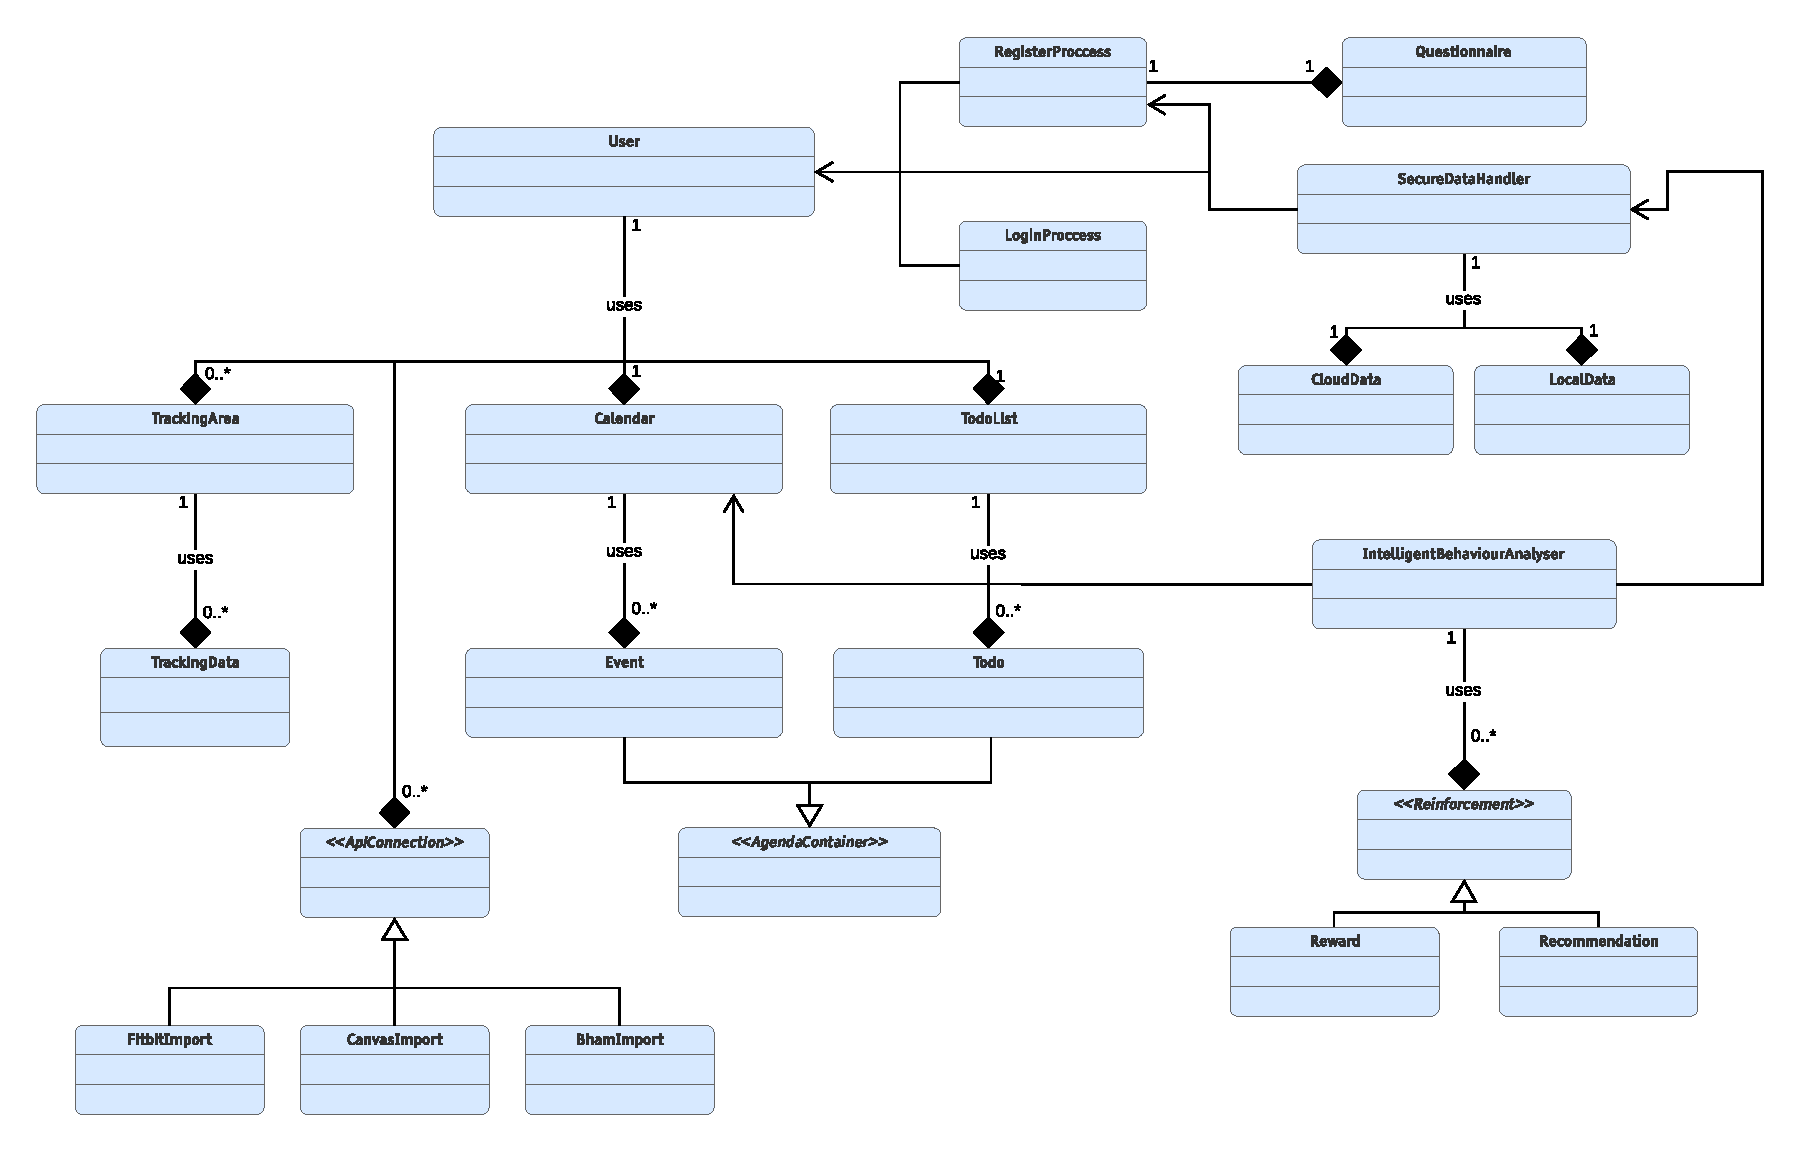
\includegraphics[angle=-90,width=0.8\textwidth]{img/Firstcut_Class_Diagram.pdf}
\end{center}
\subsection{Detailed Class Diagram}
\begin{center}
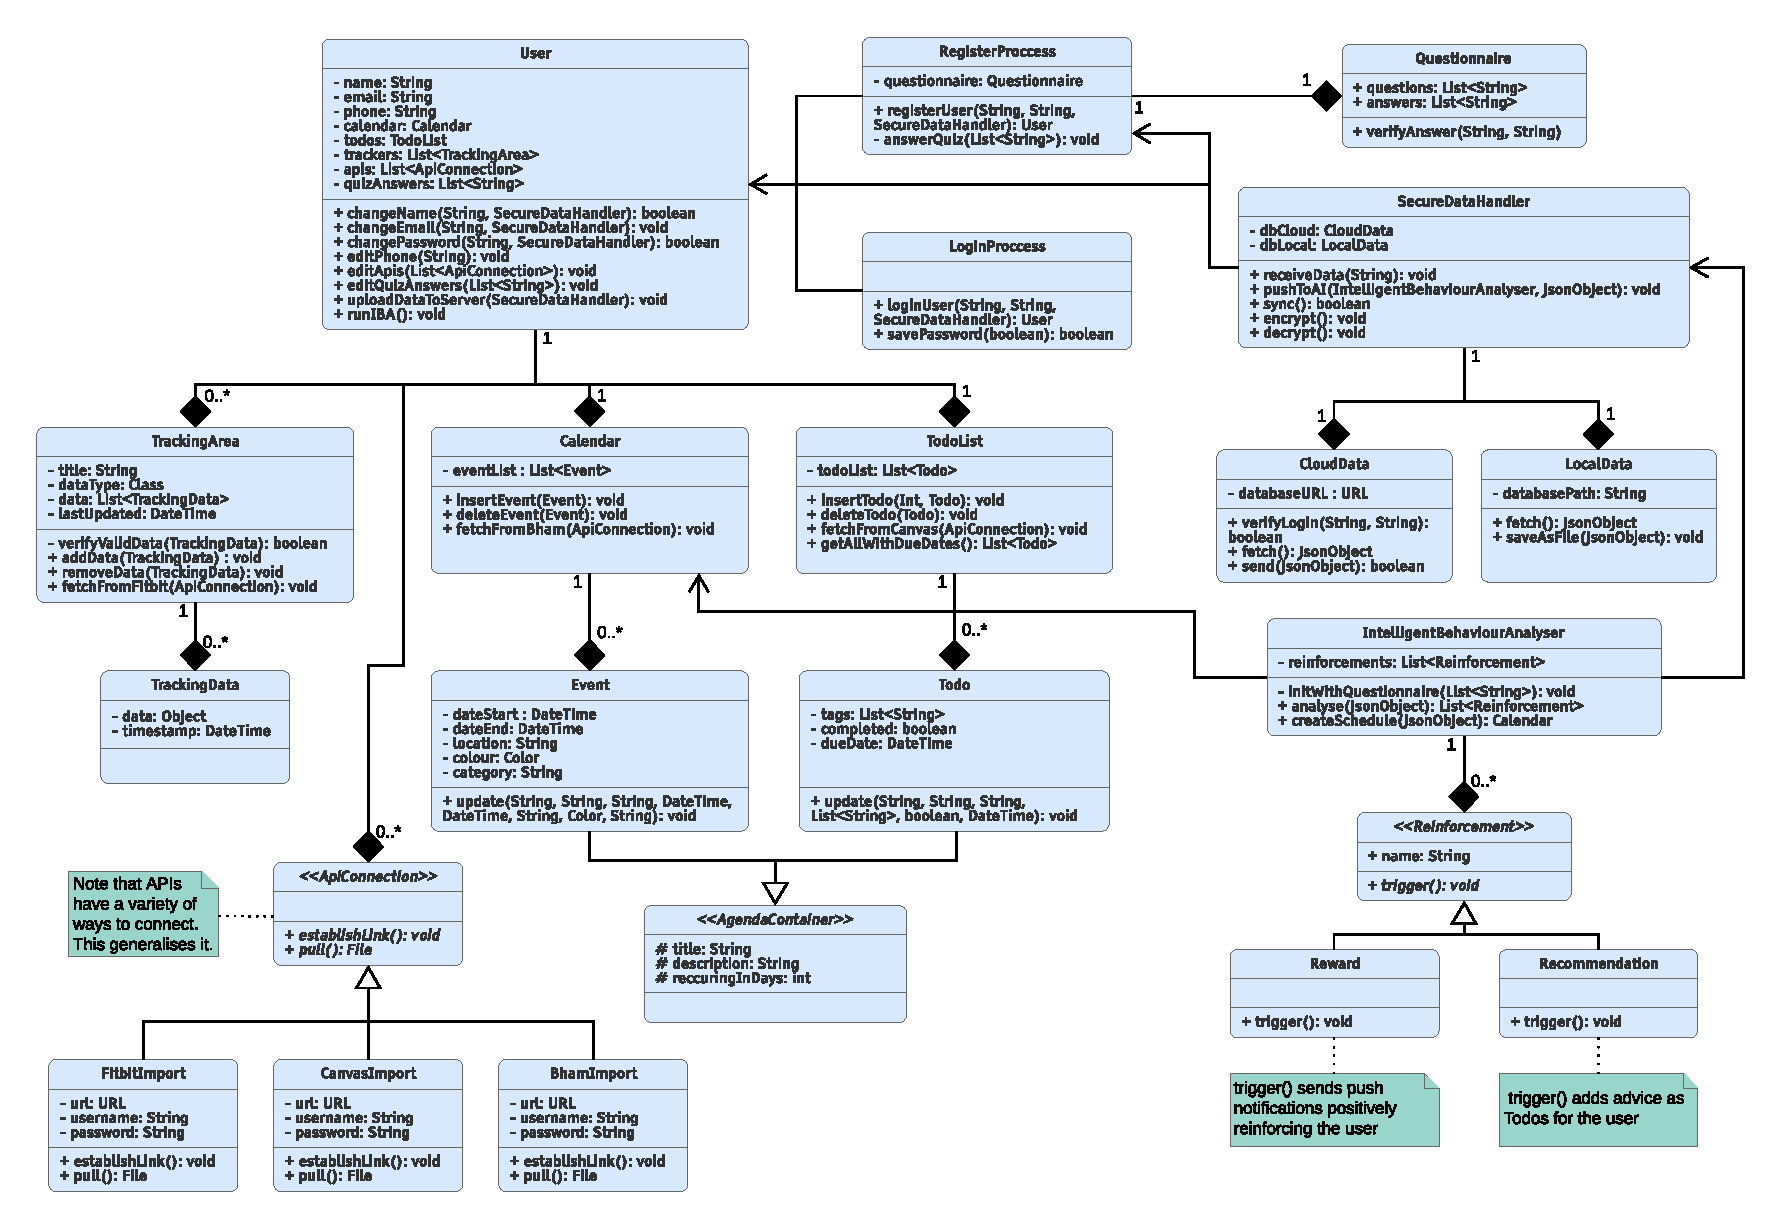
\includegraphics[angle=-90,width=0.9\textwidth]{img/Class_Diagram.pdf}
\end{center}
\newpage

\section{Object Diagram}
\begin{center}
    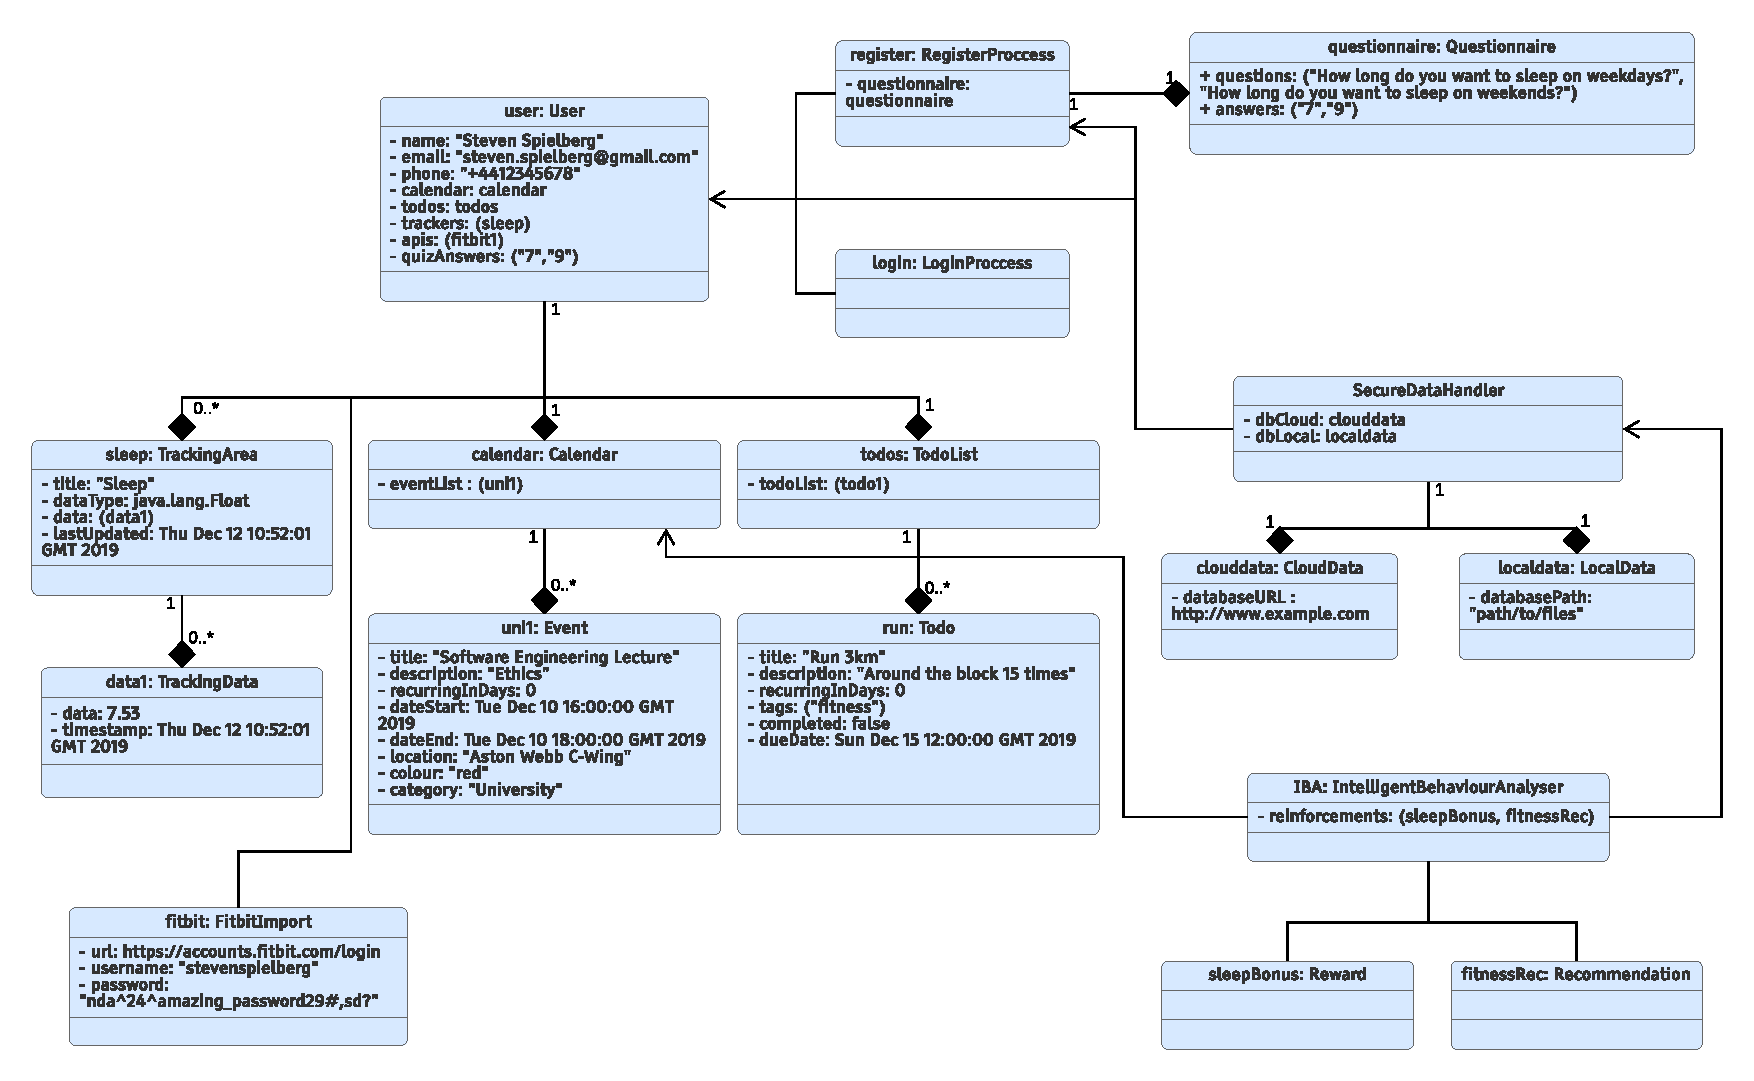
\includegraphics[angle=-90,width=0.8\textwidth]{img/Object_Diagram.pdf}
\end{center}
\newpage

\section{Sequence Diagram}
\vspace{1cm}
\begin{center}
    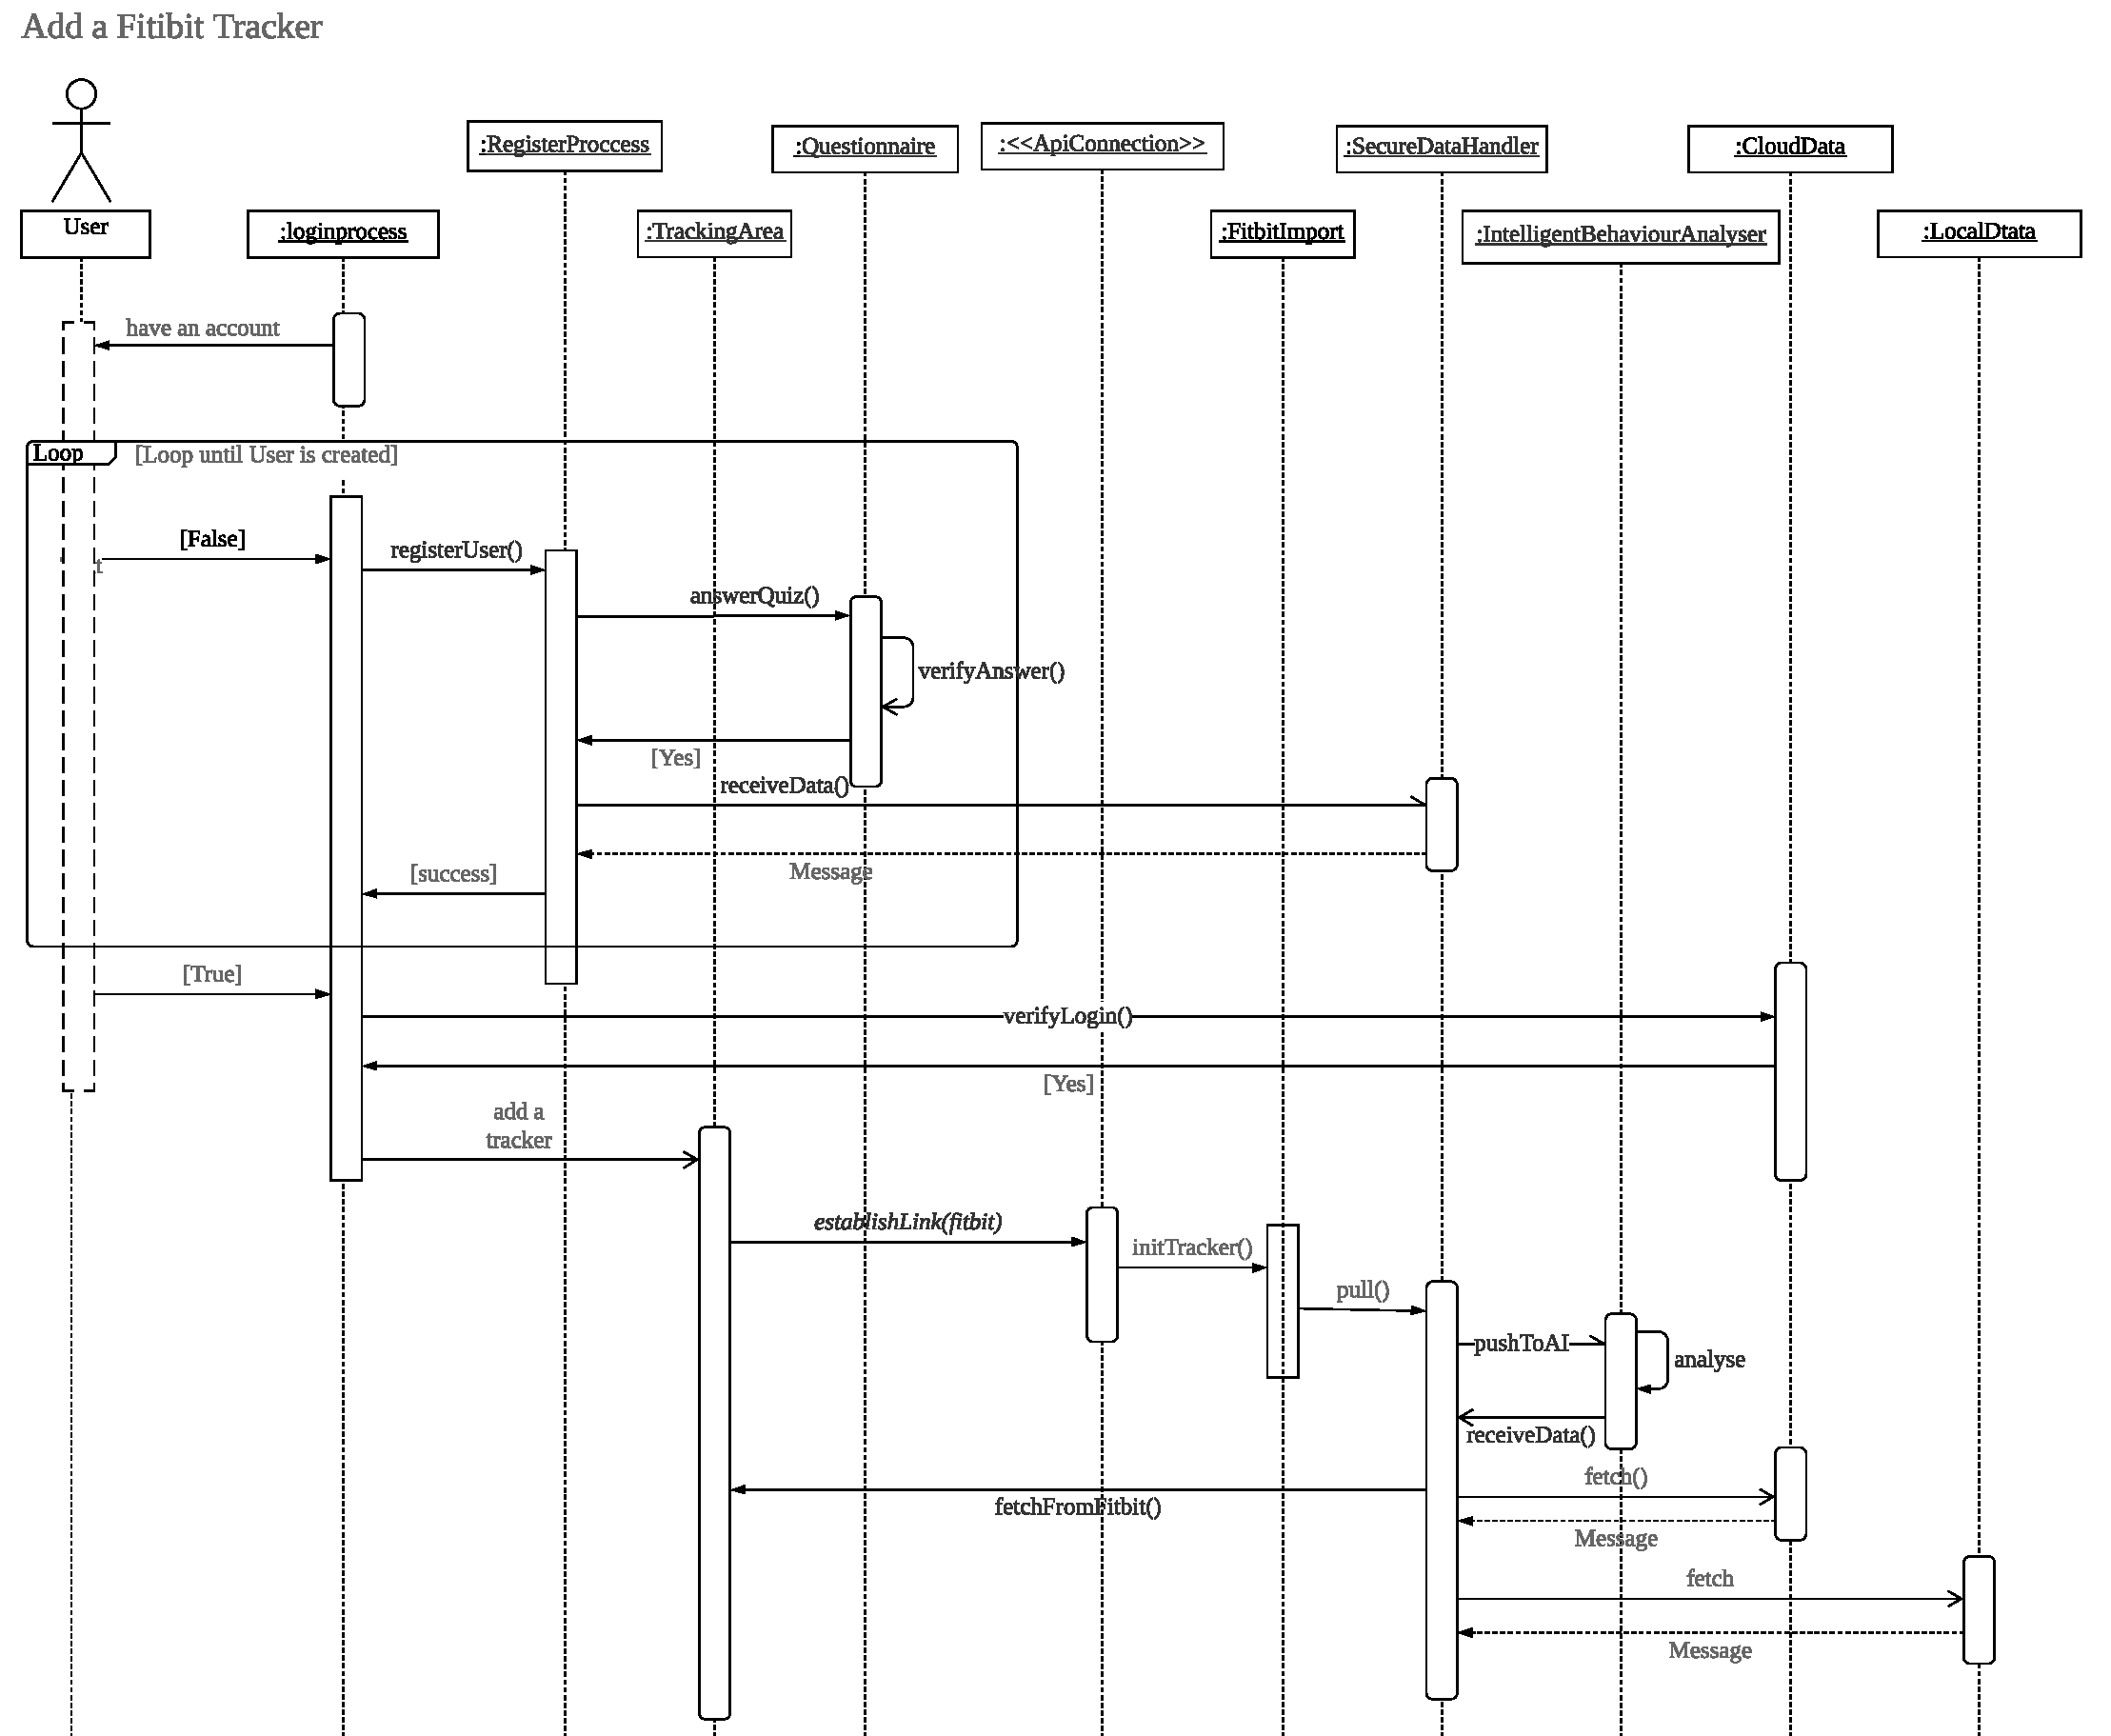
\includegraphics[angle=-90,width=\textwidth]{img/Sequence_Diagram.pdf}
\end{center}
\newpage

\section{State Diagram}
\begin{center}
    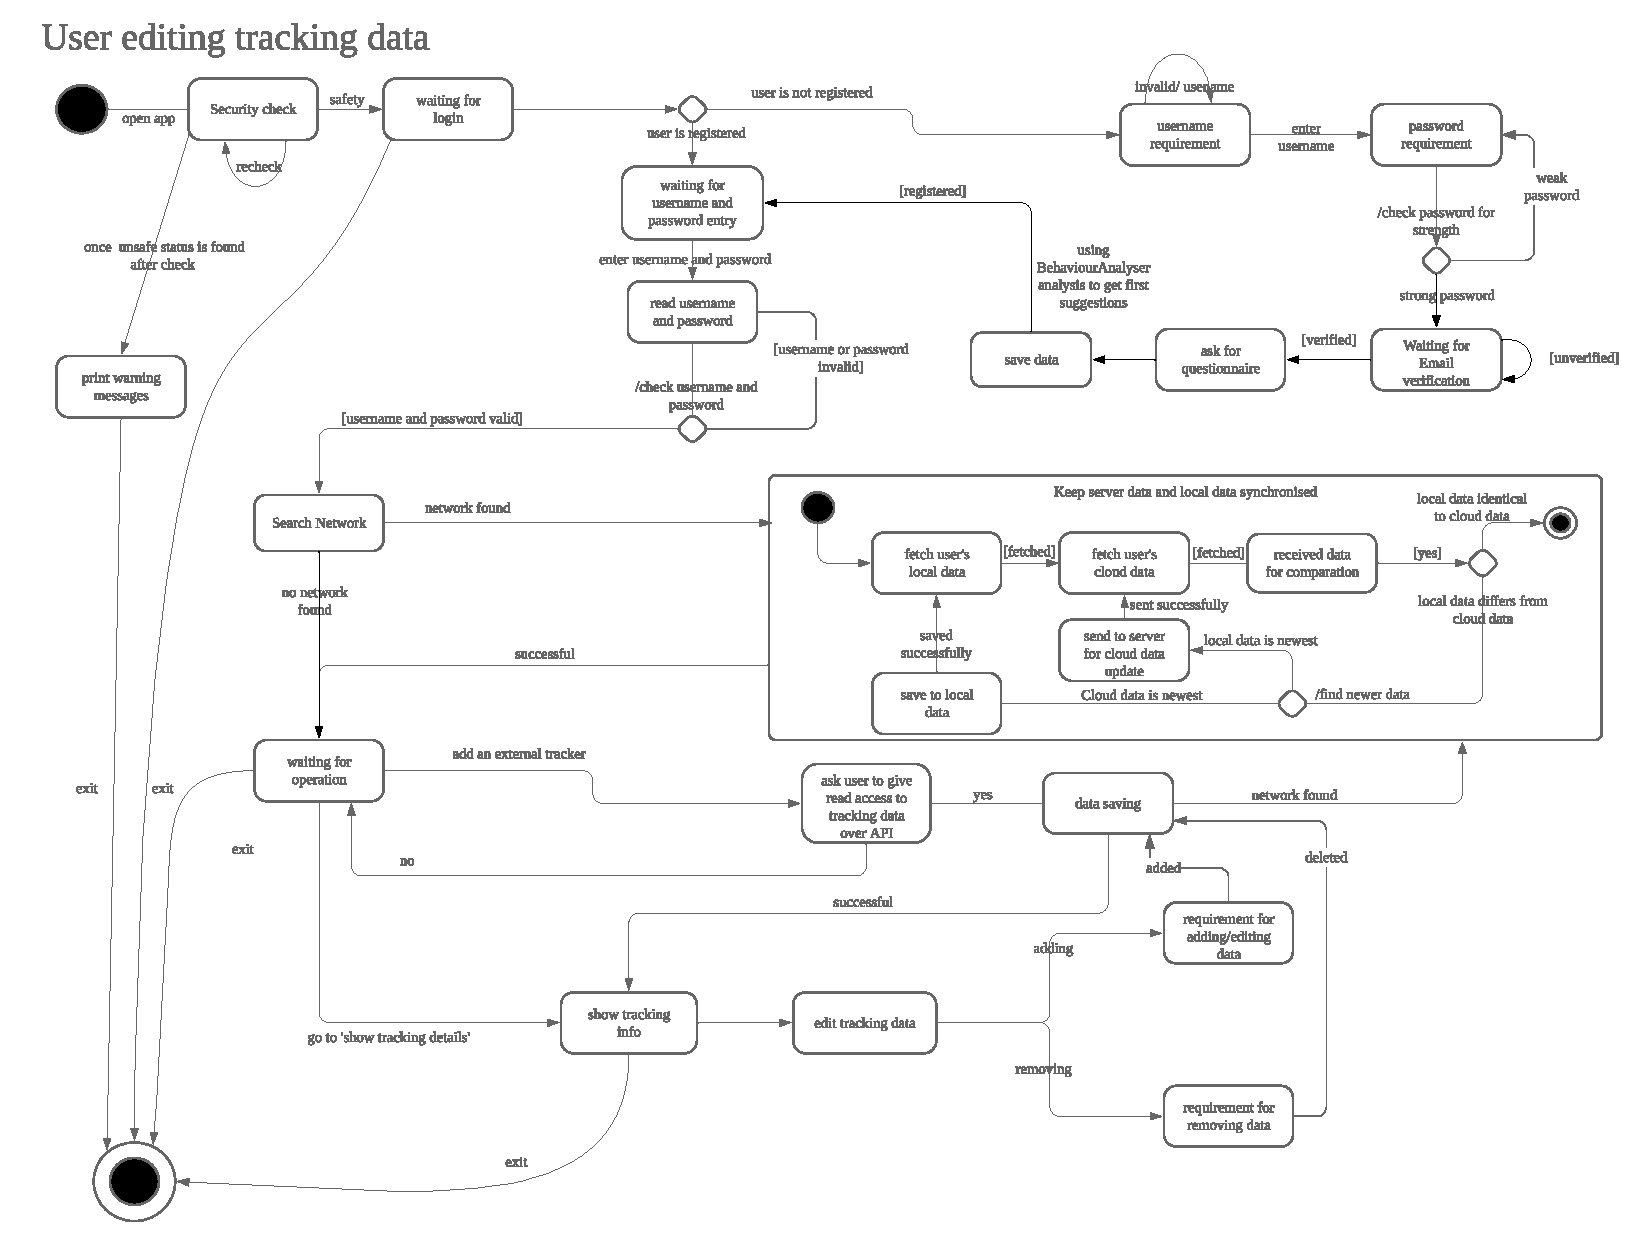
\includegraphics[angle=-90,width=\textwidth]{img/State_Diagram.pdf}
\end{center}
\newpage

\section{System Architecture}
\subsection{Component Diagrams}
\subsubsection{Candidate 1: 3-Tier Architecture}
\vspace{1cm}
\begin{center}
    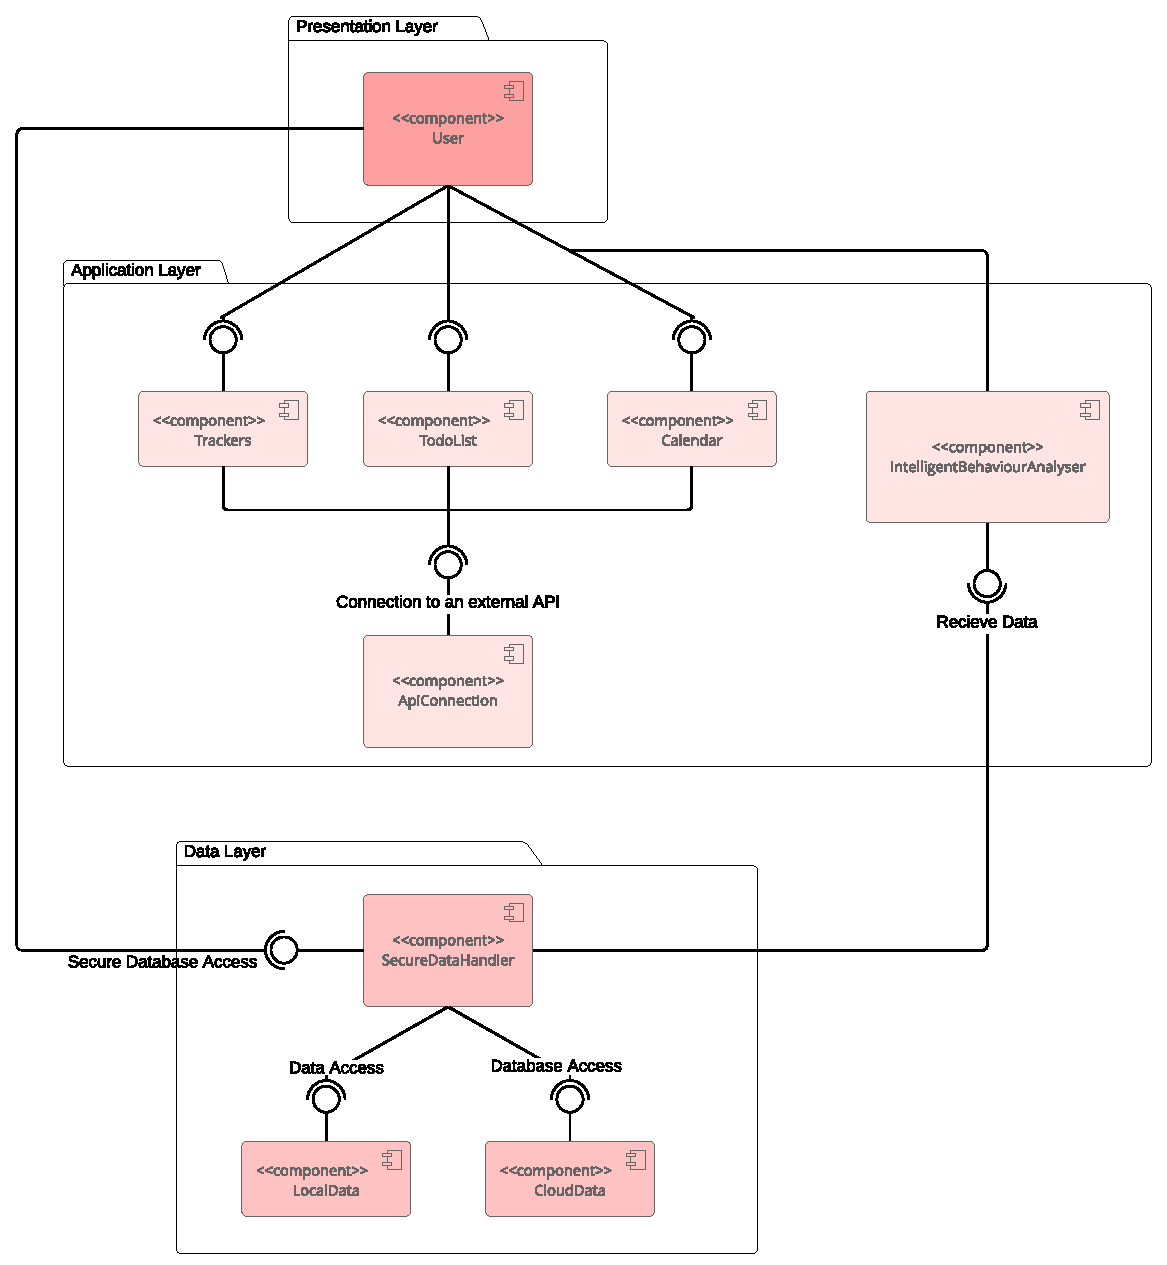
\includegraphics[width=0.9\textwidth]{img/Component_Diagram_3tier.pdf}
\end{center}
\newpage
\subsubsection{Candidate 2: Client-Server Architecture Candidate}
\begin{center}
    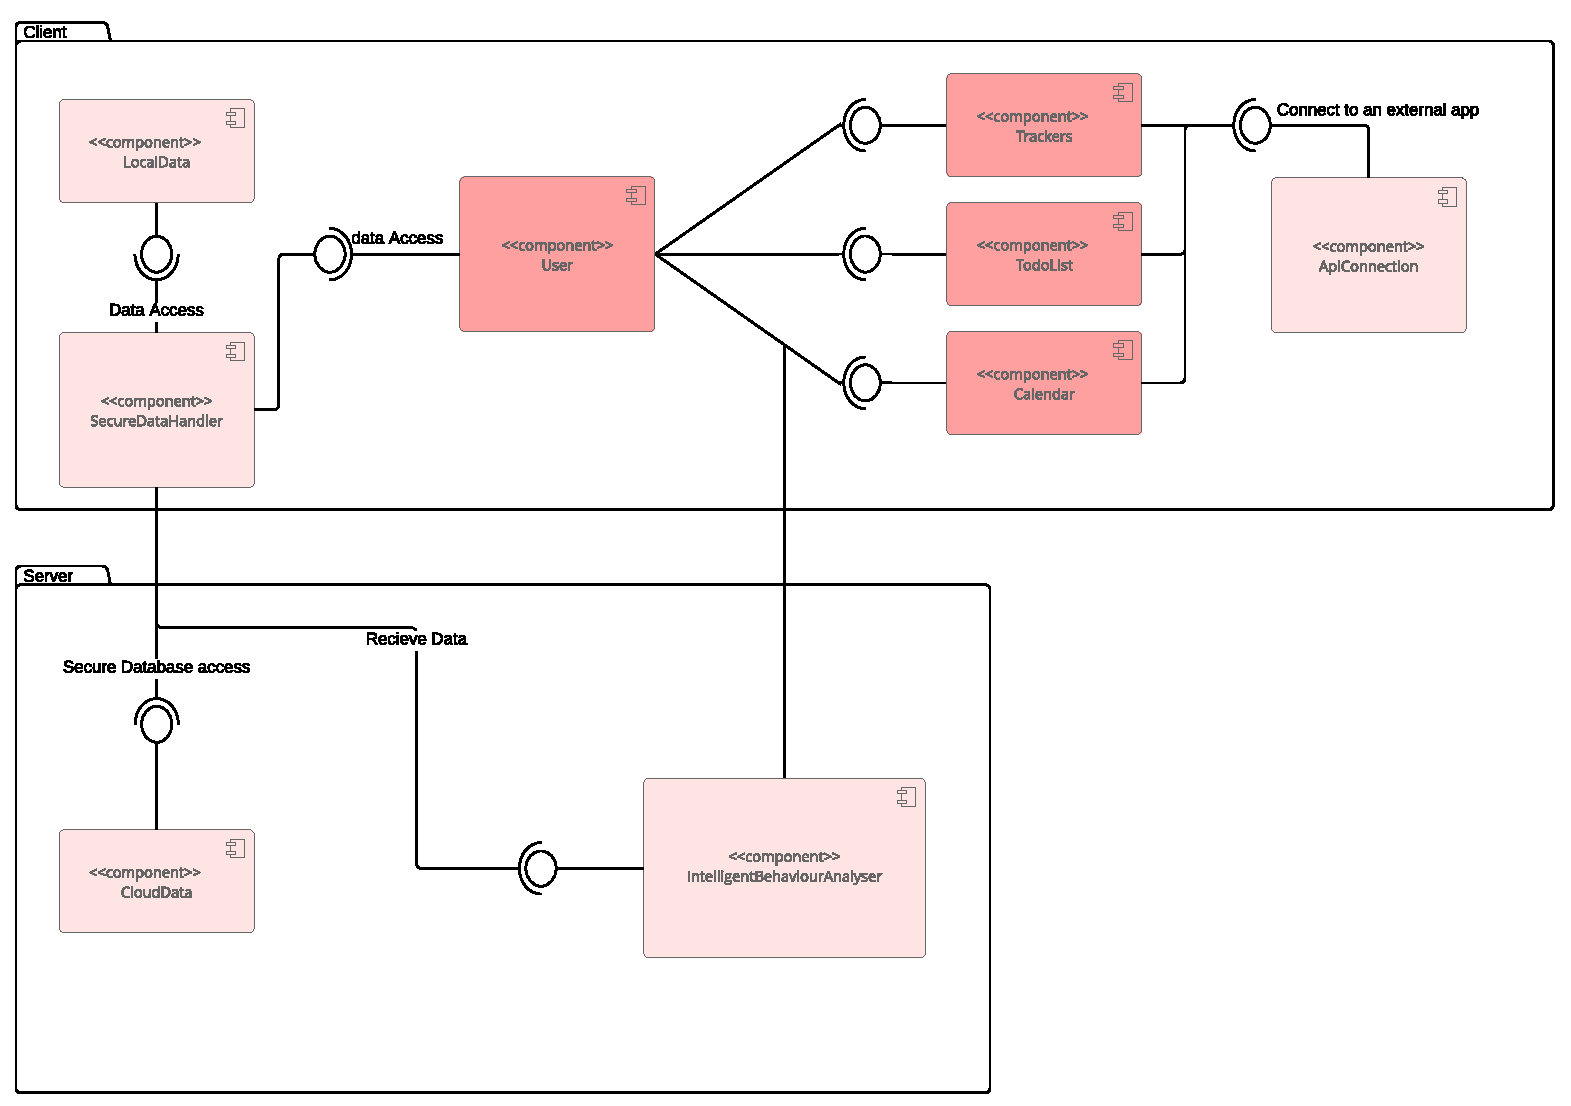
\includegraphics[width=0.9\textwidth]{img/Component_Diagram_SC.pdf}
\end{center}
\ 
\subsection{Deployment Diagram}
\begin{center}
    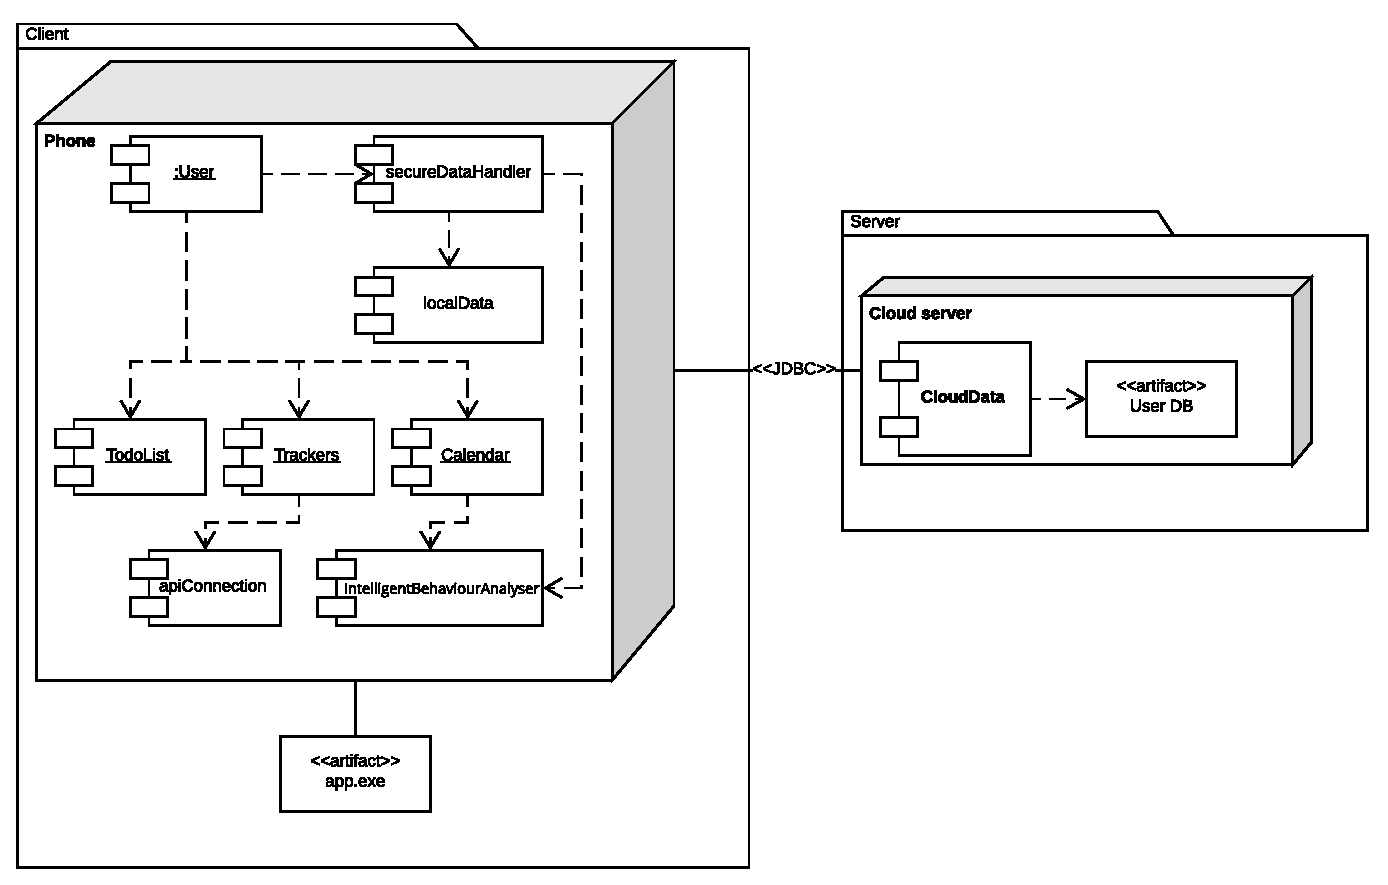
\includegraphics[width=0.9\textwidth]{img/Deployment_Diagram.pdf}
\end{center}
\newpage

\subsection{Architecture Justification}
\subsubsection{ATAM evaluation: Utility Tree}
\begin{center}
    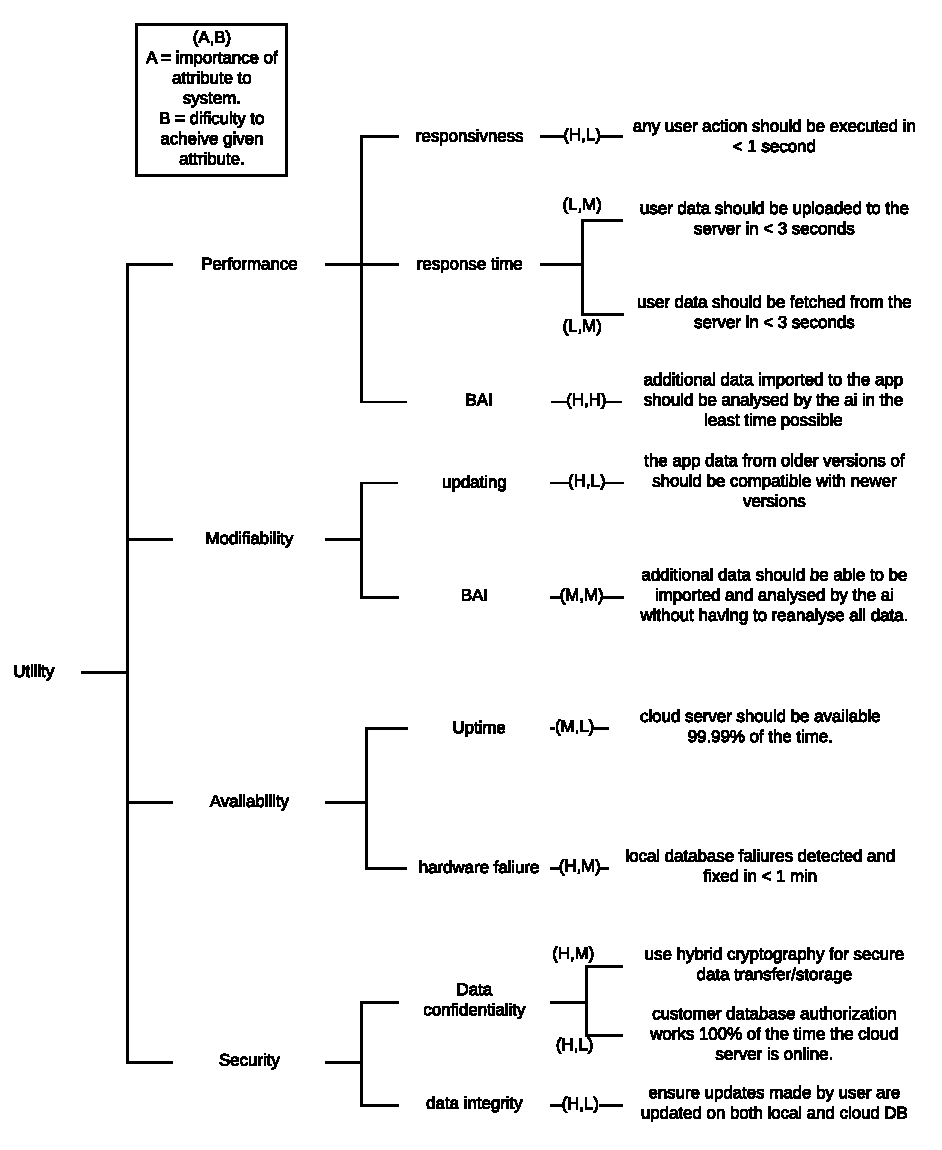
\includegraphics[width=\textwidth]{img/Utility_Tree.pdf}
\end{center}
\newpage

\subsubsection{Justification}
We will use the Two-tier \textbf{Client-Server architecture}. This is because our app is only using
the server for the database synchronisation which means there is no need for the added complications
and labor costs involved in implementing a Three tier architecture. While this can generalize and implement further
features for the system, our software would not have significant benefit as the server is only used as a remote backup.
\\
The Client-Sercer Model allows 
for faster communication to the Server because the app directly make requests to the server rather than having to go through an additional layer which
add complexity to the software. This additional \emph{feature} would slow down development where the app should be focused on quick deployment in order
to provide its service to the users in need.

Additionally the Server-Client architecture is easier to secure due to the lower complexity. Data is sent directly to and from the server so there are less 
points where data can leak, although an advantage of the three tier system would be that you are able to cache data to still access it if the servers are down.
This is mostly irrelevant to the user as he has the local data storage which is usually the most up-to-date data.
\newpage

\section{User Interface}

\subsection{Overview}
\begin{figure}[h!]
  \centering
  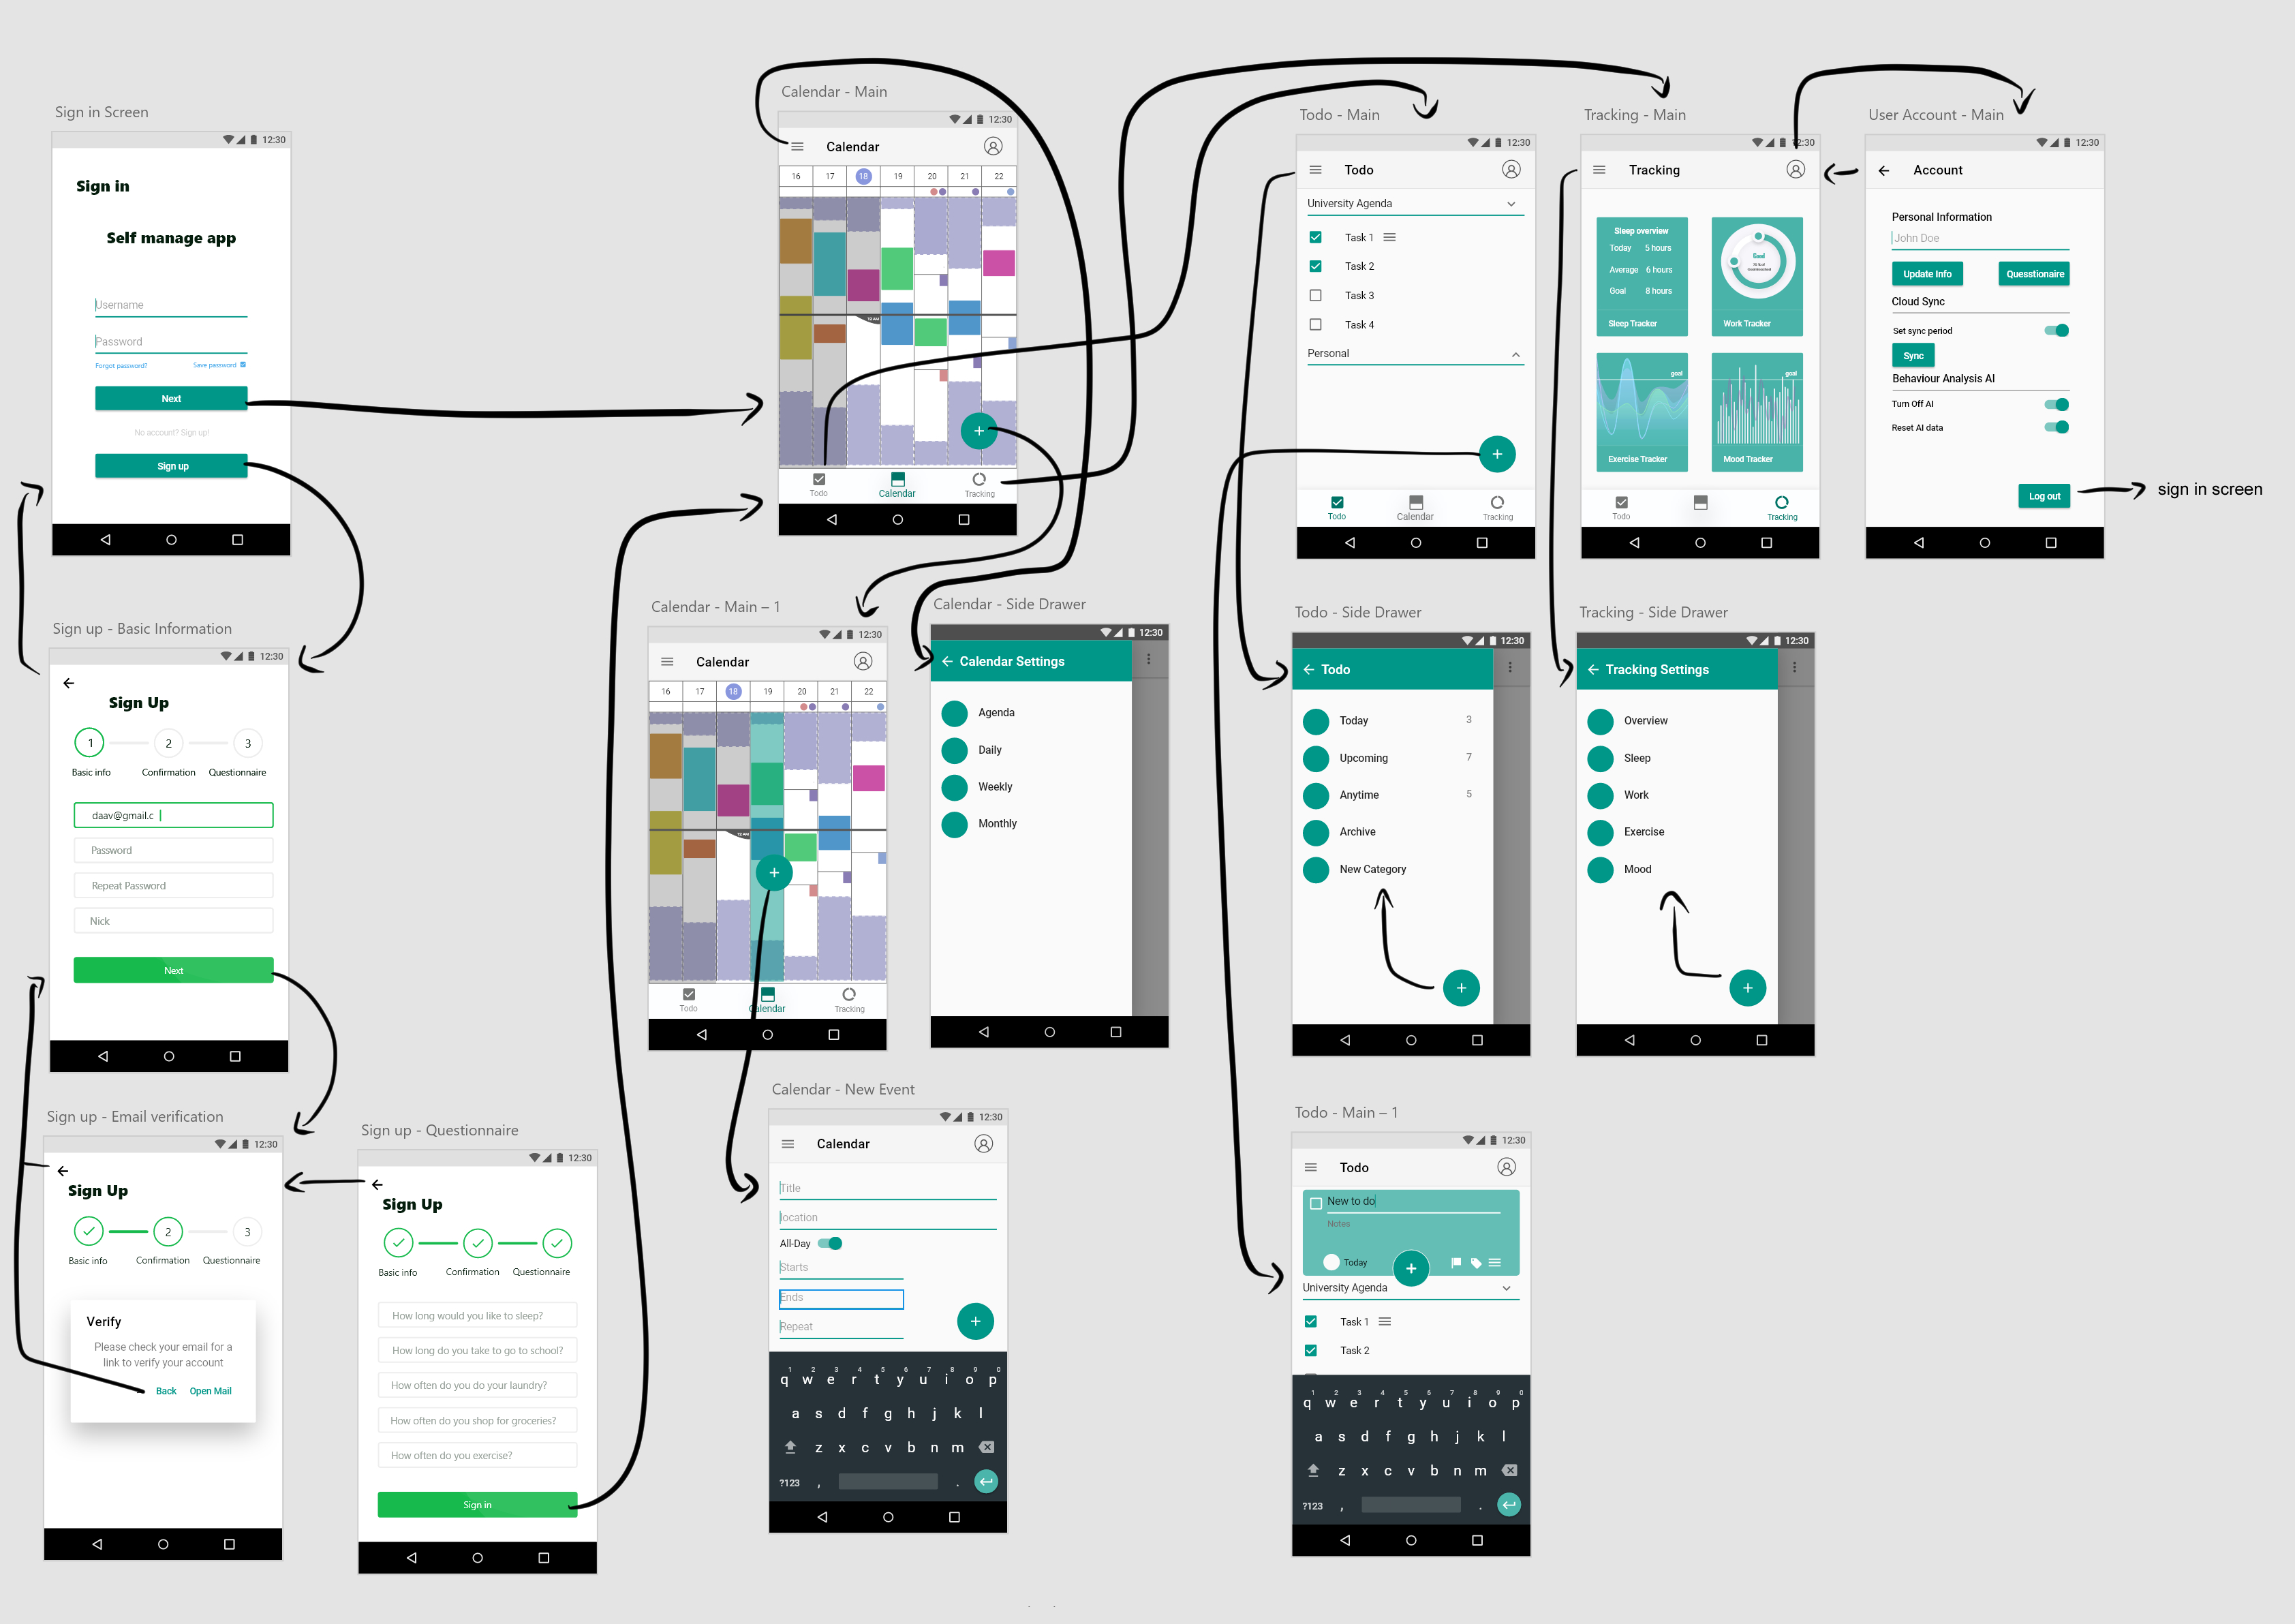
\includegraphics[angle=-90, width=0.9\textwidth]{img/ui-wireframe/Wireframe-connections.jpg}
  \caption{Overview of User Interfaces and UI action consequences}
\end{figure}
\newpage

\subsection{Login/Registration}
\begin{figure}[h!]
  \centering
  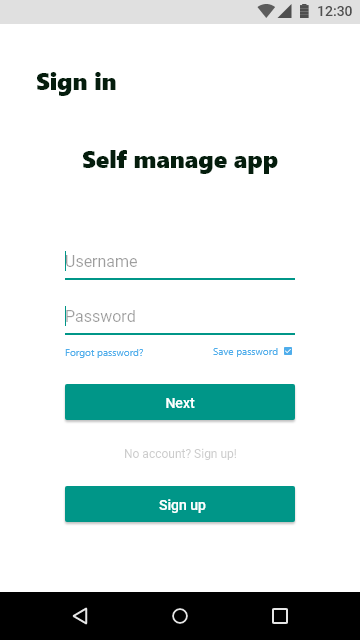
\includegraphics[width=0.75\textwidth]{img/ui-wireframe/Sign-in.png}
  \caption{Sign in}
\end{figure}
\newpage

\begin{figure}[h!]
  \centering
  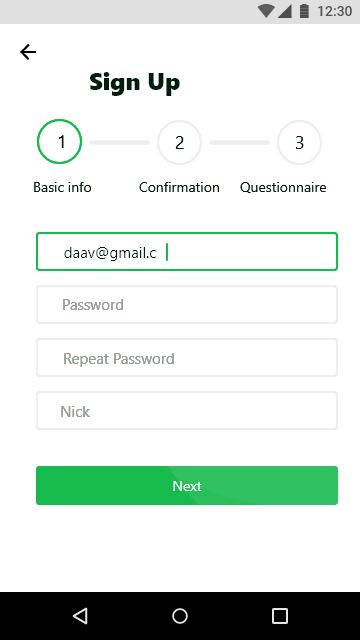
\includegraphics[width=0.75\textwidth]{img/ui-wireframe/Sign-up.png}
  \caption{Beginning of Registration process}
\end{figure}

\begin{figure}[h!]
  \centering
  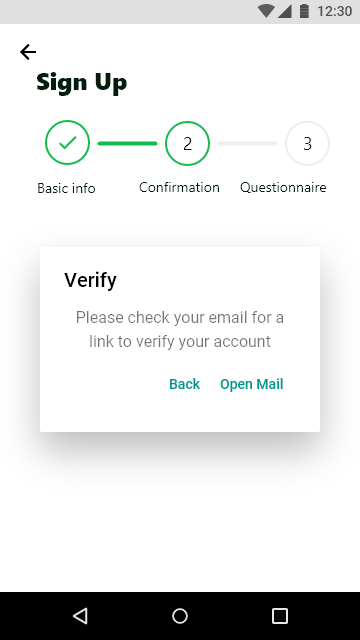
\includegraphics[width=0.75\textwidth]{img/ui-wireframe/Sign-up-verification-prompt.png}
  \caption{Verification request}
\end{figure}

\begin{figure}[h!]
  \centering
  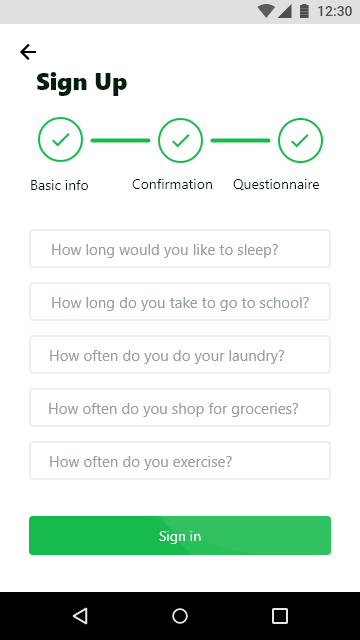
\includegraphics[width=0.75\textwidth]{img/ui-wireframe/Sign-up-questionnaire.png}
  \caption{Questionnaire}
\end{figure}
\newpage

\subsection{Calendar}
%\vspace{0.5cm}
\begin{figure}[h!]
  \centering
  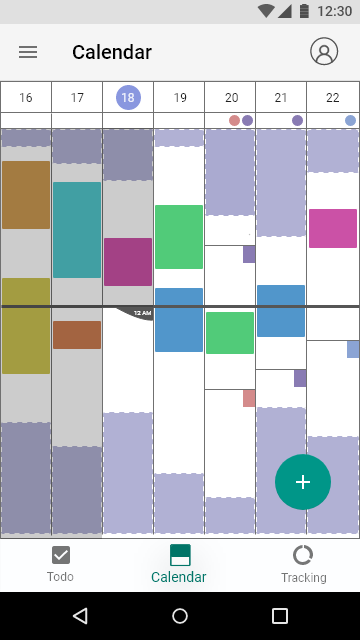
\includegraphics[width=0.75\textwidth]{img/ui-wireframe/Calendar.png}
  \caption{Weekly View mode of the Calendar tab (default page after login)}
\end{figure}
\newpage

\begin{figure}[h!]
  \centering
  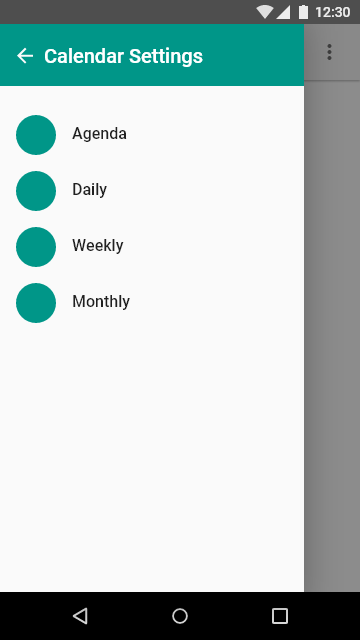
\includegraphics[width=0.75\textwidth]{img/ui-wireframe/Calendar-View.png}
  \caption{View modes of the Calendar (top left button)}
\end{figure}

\begin{figure}[h!]
  \centering
  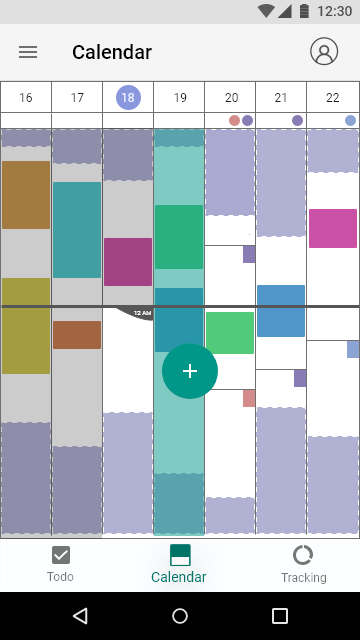
\includegraphics[width=0.75\textwidth]{img/ui-wireframe/Calendar-Add-Action.png}
  \caption{Adding an event using the draggable Plus-button}
\end{figure}

\begin{figure}[h!]
  \centering
  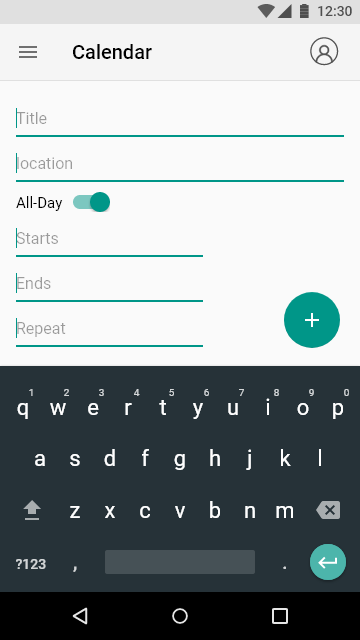
\includegraphics[width=0.75\textwidth]{img/ui-wireframe/Calendar-New-Event.png}
  \caption{Adding event data interface}
\end{figure}
\newpage

\subsection{Todo}
\begin{figure}[h!]
  \centering
  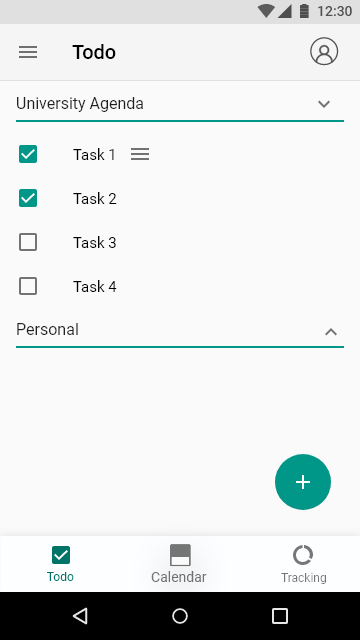
\includegraphics[width=0.75\textwidth]{img/ui-wireframe/Todo.png}
  \caption{Default Todo tab View mode}
\end{figure}

\begin{figure}[h!]
  \centering
  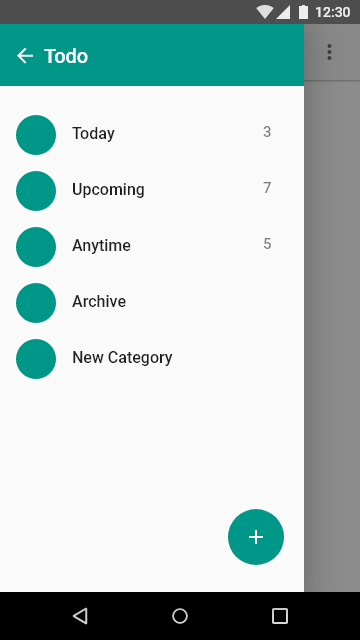
\includegraphics[width=0.75\textwidth]{img/ui-wireframe/Todo-View.png}
  \caption{View modes of the Todo interface (top left button)}
\end{figure}

\begin{figure}[h!]
  \centering
  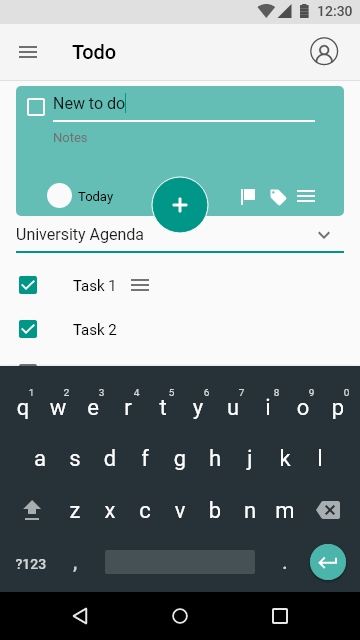
\includegraphics[width=0.75\textwidth]{img/ui-wireframe/Todo-Add-Action.png}
  \caption{Adding a ToDo using the draggable Plus-button}
\end{figure}
\newpage

\subsection{Tracking}
\begin{figure}[h!]
  \centering
  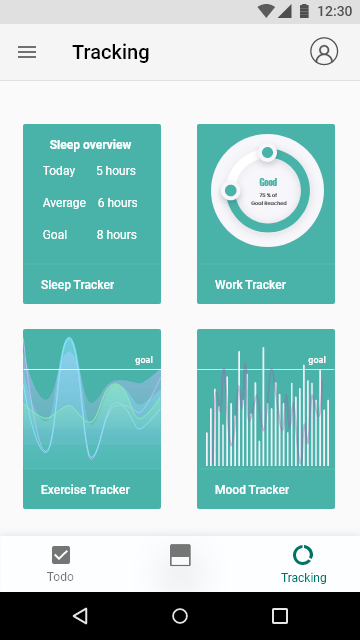
\includegraphics[width=0.75\textwidth]{img/ui-wireframe/Tracking.png}
  \caption{Default Tracking tab Overview mode}
\end{figure}

\begin{figure}[h!]
  \centering
  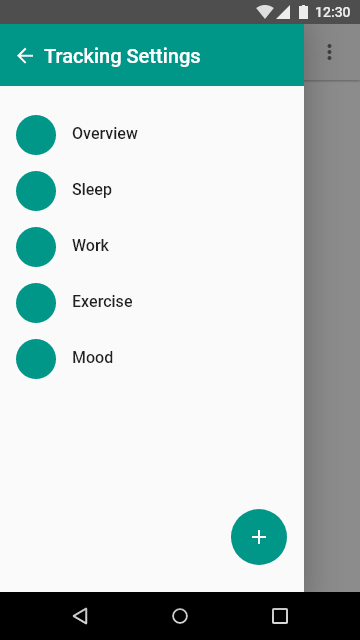
\includegraphics[width=0.75\textwidth]{img/ui-wireframe/Tracking-View.png}
  \caption{View modes of the Tracking interface (top left button)}
\end{figure}
\newpage

\subsection{Profile}
\begin{figure}[h!]
  \centering
  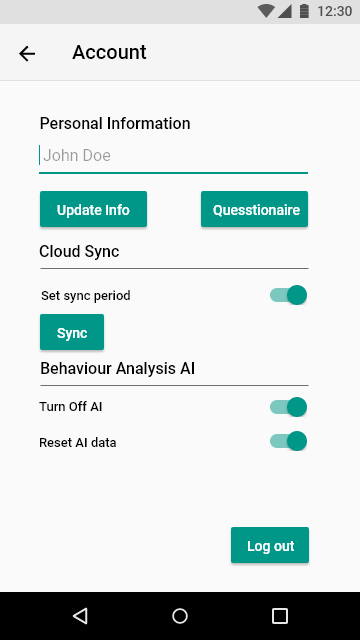
\includegraphics[width=0.75\textwidth]{img/ui-wireframe/Profile.png}
  \caption{Settings/Profile tab (top right button)}
\end{figure}
\end{document}
